% !TEX root = ../main.tex

\glsresetall

\topquote[9cm]{%
``Begin at the beginning,'' the King said gravely, \\
``and go on till you come to the end: then stop.''}%
{Lewis Carroll, \textit{Alice in Wonderland}}

{
\singlespacing
\chapter{Using rare variants to detect haplotype sharing and identity by descent}
\label{ch:sharedhap}
\minitoc
}

%
\section{Introduction}
%

\Gls{ibd} is a fundamental concept in genetics that describes the genealogical relation between individuals \citep{malecot1948mathematics}.
\N{2} chromosomes are said to be identical by descent, or rather to share a haplotype by descent, if they have inherited the same genetic material from a common ancestor \citep[\eg, see][]{Browning:2012cx,Thompson:2013cj}.
Over generations, the length of an ancestral haplotype is broken down through meiotic recombination, as the genetic material is blended with haplotypes that derive from different ancestral lineages.
Consequently, any random sample of \n{2} different chromosomes carries a unique pattern of relatedness, with different ancestries at different loci, arising as the result of historical recombination events.
The underlying structure of pairwise relatedness can be thought of as a mosaic of segments at which \n{2} chromosomes share a haplotype by descent, but where each of these IBD segments traces back to a different \gls{mrca}.

In general, knowledge about relatedness, haplotype sharing by descent, or the recombination history of a sample is of importance in a variety of statistical operations that are used in both population and medical genetics research \citep{Milligan:2003bd,Albrechtsen:2009cb,Gusev:2009hd}; for example, to provide insights into the demographic history of a population \citep{Harris:2013id}, to inform methods for genotype phasing and imputation \citep{Kong:2008gh}, to map disease loci using linkage analysis \citep{Purcell:2007dg,Albrechtsen:2009cb}, as well as to reveal patterns of population stratification and to identify unreported relatedness among individuals in disease association analysis \citep{Freedman:2004dk,Price:2006cd,Choi:2009fm,Mathieson:2012hb}.

The entire IBD structure of a sample can be represented by the \gls{arg} \citep{Griffiths:1991jp,Griffiths:1996dx,griffiths1997}, which is straightforward to generate in coalescent simulations, but inference from observed data is limited \citep{Rasmussen:2014cq}.
This is because even complete data is unlikely to provide sufficient information to explicitly infer the \gls{arg}, in addition to the problem that inference becomes computationally expensive for larger sample sizes.
%The general problem remains that recombination events do not leave direct traces and need to be estimated from available data.
Most methods for IBD discovery operate on summary statistics to make inference computationally tractable.

In practice, IBD discovery is largely dependent on the length of a shared haplotype and the genetic similarity between compared sequences.
Co-inherited haplotypes that are separated by only a few meioses are expected to cover relatively long tracts, because recombination had less time to break down the length of the region shared between the \n{2} chromosomes \citep{Thompson:2008cub,Thompson:2013cj}.
Likewise, as mutations are accumulated along different genealogical lineages, the similarity between shared segments is expected to decrease over time.
%, such that haplotype frequencies are seen as being statistically independent.
Thus, for most purposes, the detection of \emph{recent} IBD is of primary interest \citep{Browning:2010dz}.

Numerous approaches for the detection of IBD segments have been proposed, most of which attempt to infer IBD based on measures of genetic similarity or through use of statistical models to determine salient patterns of \gls{ld}.
Commonly employed tools are
\texttt{PLINK} \citep{Purcell:2007dg},
\texttt{GERMLINE} \citep{Gusev:2009hd},
\texttt{fastIBD} \citep{Browning:2011do}, and
\texttt{Refined\,IBD} \citep{Browning:2013eh}, to name a few.
The methodological diversity of existing approaches emphasises the central role of IBD in genetics, but also indicates that there is a need for an accurate as well as efficient method to detect IBD in larger samples of purportedly unrelated individuals.

Due to the growing magnitude of available genomic datasets, IBD discovery is becoming more computationally expensive.
Note that alternate approaches exist, for example methods to perform \gls{lrp} implicitly harness long IBD regions among related individuals \citep{Kong:2008gh,Palin:2011cl,loh2016fast}, which employ  computationally efficient methods to match relatively long (\eg $>$\SI{10}{\centi\morgan}) haplotypes even in very large datasets.
But in a general context, as IBD describes a pairwise relationship between \n{2} haplotypes, a search algorithm may visit each of the possible pairs of chromosomes in a sample to determine IBD status from patterns of shared genetic variation observed along the full length of the chromosome.
For instance, in a sample of $n$ chromosomes, there are ${{{n}\choose{2}} = \rfrac{n(n-1)}{2}}$ possible pairs that need to be scanned to resolve IBD status if done in an exhaustive manner.
To reduce this search space, it would be convenient if a pairwise approach could be targeted to regions and individuals for whom it is more likely to find recent haplotype sharing by descent.

In this chapter, I present a non-probabilistic method to detect IBD segments in pairs of diploid individuals, which utilises rare variants as indicators of recent relatedness.
The computational burden of IBD detection is thereby reduced due to the relative low number of individuals that share a given rare or low-frequency allele.
In each pair, the regions to each side of a focal allele are scanned, so as to infer the ``breakpoints'' of historical recombination events that delimit the underlying IBD segment.
The inference of recombination is based on the \emph{four-gamete test} by \citet{Hudson:1985wh}, for which haplotype information is required, but which is extended, following \citet{Mathieson:2014ig}, such that recombination breakpoints can be inferred in genotype data.

In the following section, I highlight the genealogical properties of rare variants which make them useful for the inference of recent and relatively long haplotypes by descent.
I then describe the method by which IBD segments are detected, conditional on variation observed at a focal rare variant.
\Delete{In addition, I present a simple approach to infer the shared haplotype sequence from genotype data.}
For the evaluation of the methodology presented, I generated a large dataset using coalescent simulations, so as to measure the accuracy of the IBD detection method in comparison to the true IBD structure (determined from simulation records).
These results are also compared to IBD detected using an alternate method.
Lastly, I apply the method presented in this chapter to data from the \glsentryfull{1kg}.


%
\section{Rare variants as indicators of haplotype sharing by descent}
\label{sec:rarevars}
%

One of the properties of rare variants is their presumed young age, as a low frequency is indicative of a recent origin through mutation; \ie the frequency of an allele is assumed to be a proxy to its age \citep{Kimura:1973ug,Griffiths:2013ec}.
Individuals that share a rare allele are therefore likely to have a relatively long chromosomal segment co-inherited from a common ancestor.
For example, genetic markers tend to be in high \gls{ld} with alleles at lower frequencies, because the alleles near a rare variant site are likely to segregate together on the same haplotype \citep{Kruglyak:1999dp,Slatkin:2008ks}.

To explain the relation between IBD length and age, consider a focal site at which \n{2} haplotypes are shared by descent.
The length of the IBD segment is defined by the nearest ancestral recombination events that have occurred to either side of the focal position; \ie haplotype sharing is broken down by recombination on both sides independently.
The expected length of the IBD segment is determined by the number of meioses that separate \n{2} haplotypes in relation to the \gls{mrca} who lived $t$~generations in the past; hence, the pair is separated by ${2 t}$~meioses.
In each meiosis, recombination is modelled as a Poisson process with rate of~1 per unit of genetic distance (\emph{Morgan}).
It follows that the recombination process over ${2 t}$~meioses is Poisson distributed with rate equal to ${2 t}$.
The expected length can be expressed as the sum of \n{2} independent random variables that are exponentially distributed, and which describes the distance to either side of the focal position \citep[see][]{Wakeley2016book}; \ie the length, $L$, is gamma-distributed with shape~$2$ and rate~${2 t}$, namely ${L \propto \Gamma(2, 2 t)}$.

%
%!TEX root = ../../main.tex


\begin{figure}[!htb]
\centering
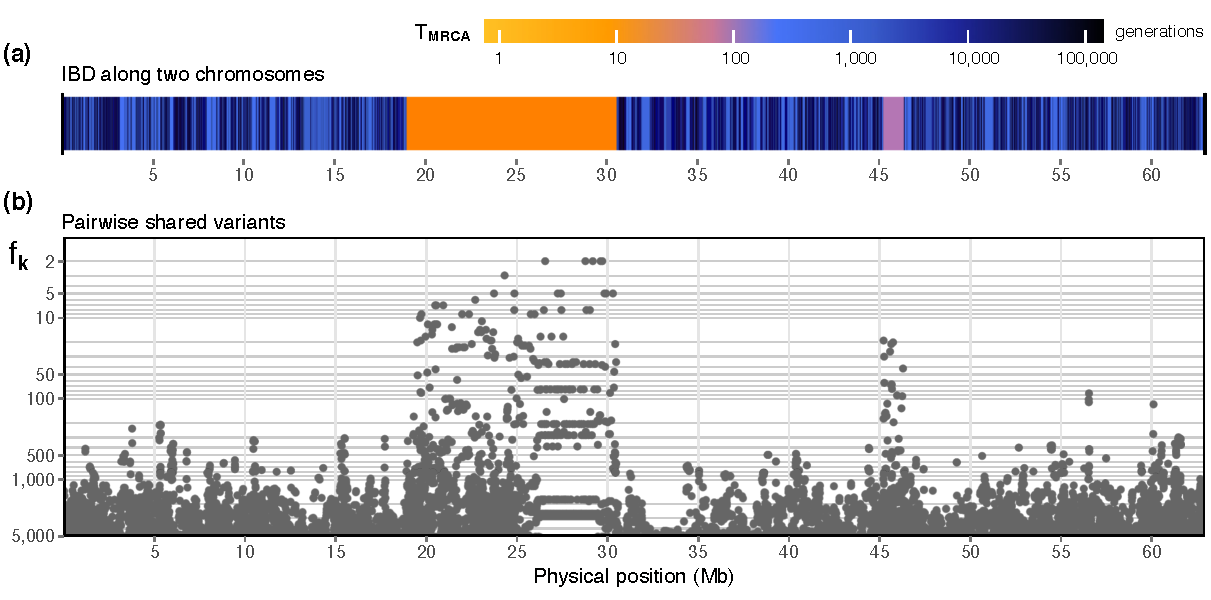
\includegraphics[width=\textwidth]{./img/ch3/pair_ibd_example}
\Caption{IBD structure and pairwise variant sharing}
{A dataset of ${N=\num{5000}}$ haplotypes was simulated under the coalescent using \texttt{msprime} \citep{Kelleher:2016fn}.
IBD status was determined from simulated genealogies for a pair of chromosomes selected at random from the set of chromosomes that shared a rare allele (frequency $\leq 0.5\%$).
Panel~\textbf{(a)} shows the ``mosaic'' of IBD segments along the full length of the simulated region for the \n{2} selected chromosomes.
The length of a given IBD segment is defined by the chromosomal interval over which the \gls{mrca} of the selected pair does not change.
The colour of each segment indicates the \gls{tmrca} for the selected pair.
Panel~\textbf{(b)} shows the physical position of \fk{} variants shared by the \n{2} chromosomes, ranging from very low allele frequency at the top (\fk{2}) to very high frequency at the bottom (\eg~\fk{>500}).
Note that the simulation was carried out under variable recombination rates using the genetic map for human chromosome~20 from the \glsentryfull{hapmap} Phase~\rom{2} Build~37.
The pattern of extended shared variation seen at positions around 25--30~\gls{Mb} arises from a low recombination rate at the region of the centromere.}
{fig:pair_ibd_example}
% \vspace{-5pt}
% \hrulefill%
\end{figure}

\glslocalresetall

%

Given this exponential ``decay'' of IBD length over time, rare or low-frequency variants are useful for identifying genomic regions in which individuals are likely to share recent and relatively long IBD tracts.
For example, \citet{Mathieson:2014ig} selected doubletons (alleles that are present only twice in a sample), which they refer to as \fk{2} variants, to identify the shared haplotype in the \n{2} individuals sharing the allele.
To borrow from this notation, henceforth, \fk{} is used to denote a variant at which $k$ allele copies are found in a sample.

To emphasise the utility of rare variants, see the example shown in \cpref{fig:pair_ibd_example}.
Using coalescent simulations, a sample of ${N = \num{5000}}$ chromosomes was generated.\footnote{See \cpref{sec:msprime} for a description of how data were simulated.}
A rare variant was randomly selected (frequency $\leq 0.5\%$), as well as \n{2} of the chromosomes which share the focal allele.
The underlying IBD structure for the given pair of chromosomes was determined from simulation records and shown in \cref{fig:pair_ibd_example}{a}.
IBD segments are distinguished by the \glsentryfull{tmrca} at each position along the sequence.
To illustrate pairwise allele sharing, \Correct{the} frequency of each allele shared by the \n{2} haplotypes is shown by chromosomal position in alignment with the IBD structure above; see \cref{fig:pair_ibd_example}{b}.
As suggested in the figure, the majority of low-frequency variants align with IBD segments that are more recent.

%
%!TEX root = ../../main.tex


\begin{figure}[p]
\makebox[\textwidth][c]{%
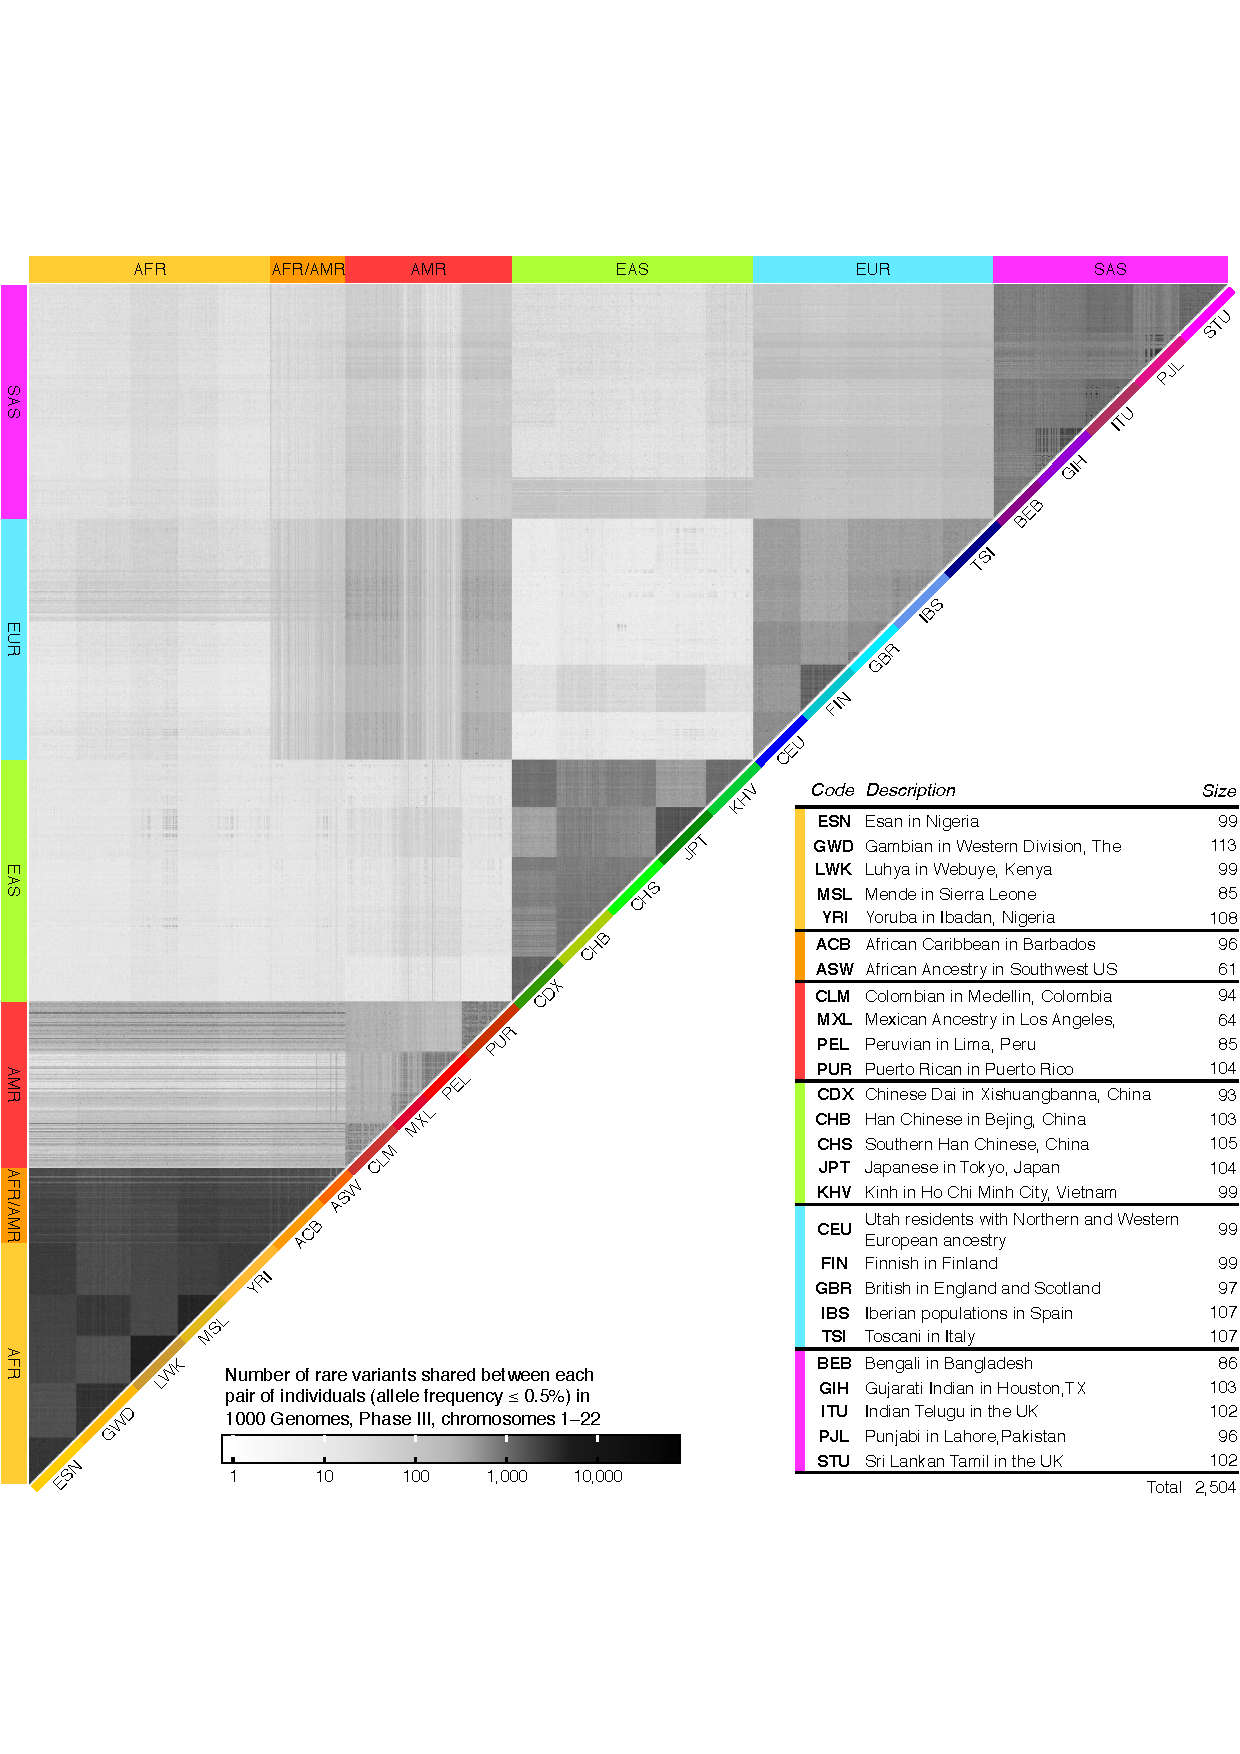
\includegraphics[width=1.1\textwidth]{./img/ch3/popstruct_1kg}%
}
\Caption{Rare variant sharing in the 1000 Genomes dataset}
{The plot shows the upper triangle of a pairwise sharing matrix in which the number of variants shared in each pair of individuals is indicated by tones of grey (log-scaled), ranging from \emph{light} (low number) to \emph{dark} (high number); see legend.
Pairwise rare variant sharing was determined for all shared alleles observed at  frequency ${\leq 0.5\%}$, across chromosomes 1--22, and in each pair of the \n{2504} individuals present in the final release dataset of the \glsentrylong{1kg} Phase~\rom{3}.
The dataset comprises sample data from \n{6} continental populations (or \emph{super-populations}) which are further subdivided in \n{26}~populations of different ethnic background.
Each group is abbreviated using a \n{3}-letter code.
The \n{6} continental populations are defined as follows;
African~(AFR), African-American~(AFR/AMR), American~(AMR), East~Asian~(EAS), European~(EUR), and South~Asian~(SAS).
The table in the lower right corner shows the code and description of each  population sample, as well as the number of individuals in each group.}
{fig:popstruct_1kg}
\end{figure}

%

The majority of variants observed in the human genome are low in frequency or rare.
For example, there are \Value{84.7}~million \glspl{snp} in the final release dataset of the \gls{1kg} Phase~\rom{3} (${N = \num{2504}}$), of which \Percent{71.93193} are below 1\% allele frequency and \Percent{64.2427} are below 0.5\% (after removing singletons and monomorphic sites), suggesting that there are ample opportunities to find rare allele sharing.
This is illustrated in \cpref{fig:popstruct_1kg}, which indicates the number of alleles shared between each pair in the dataset (chromosomes~1--22), at allele frequency~${\leq 0.5\%}$.
Notably, the sharing pattern highlights population structure, as the number of shared alleles is generally larger within a sub-population.



%
\section{IBD detection around rare variants}
\label{sec:tidy}
%

In the following sections, I describe the methodology by which IBD segments are detected around rare variant sites.
I then describe the implementation of each of the \n{2} tests for the detection of IBD segments in large sample data.
Lastly, I conclude this section by highlighting certain caveats of the implemented method before its evaluation using simulated data.


%
\subsection{Inference of historical recombination events}
%

\N{2} approaches for a non-probabilistic inference of recombination events are described below; these are the \emph{\acrlong{fgt}} \citep{Hudson:1985wh}, which requires haplotype information, and the criterion of \emph{inconsistent homozygote genotypes} \citep[see][]{Mathieson:2014ig}, which requires genotype data; henceforth referred to as the \emph{\acrlong{dgt}}.
\Addition{Note that the aim of this implementation is to detect recombination in pairs of diploid individuals, relative to a given target position in the genome.}

\paragraph{\Gls{fgt}.}
Given \n{4} haplotypes in \n{2} diploid individuals, a recombination event is inferred between \n{2} loci if all \n{4} possible gametes are observed.
This holds true under the infinite sites model \citep{Kimura:1969tn}, where mutation events may only occur once per site in the history of a sample, such that at most \n{2} allelic states can be observed at a given site.
It follows that for a pair of sites there are \n{4} possible allelic state configurations; ${(0,0)}$, ${(0,1)}$, ${(1,0)}$, and ${(1,1)}$, where 0 and 1 denote the ancestral and derived type, respectively.
If all \n{4} configurations are observed, genealogies at the \n{2} sites are incompatible and the observation can only be explained by a recombination event that occurred in the history of the sample.
Because recurring mutations or back mutations are assumed to have zero probability, at least \n{1} recombination event must have occurred in the interval between the \n{2} sites.
In the following, the term \emph{breakpoint} is used for either of the \n{2} sites that together delimit the interval.
An example configuration is shown in \cpref{fig:info_fgt}.

%
%!TEX root = ../../main.tex


\begin{figure}[!htb]
\centering
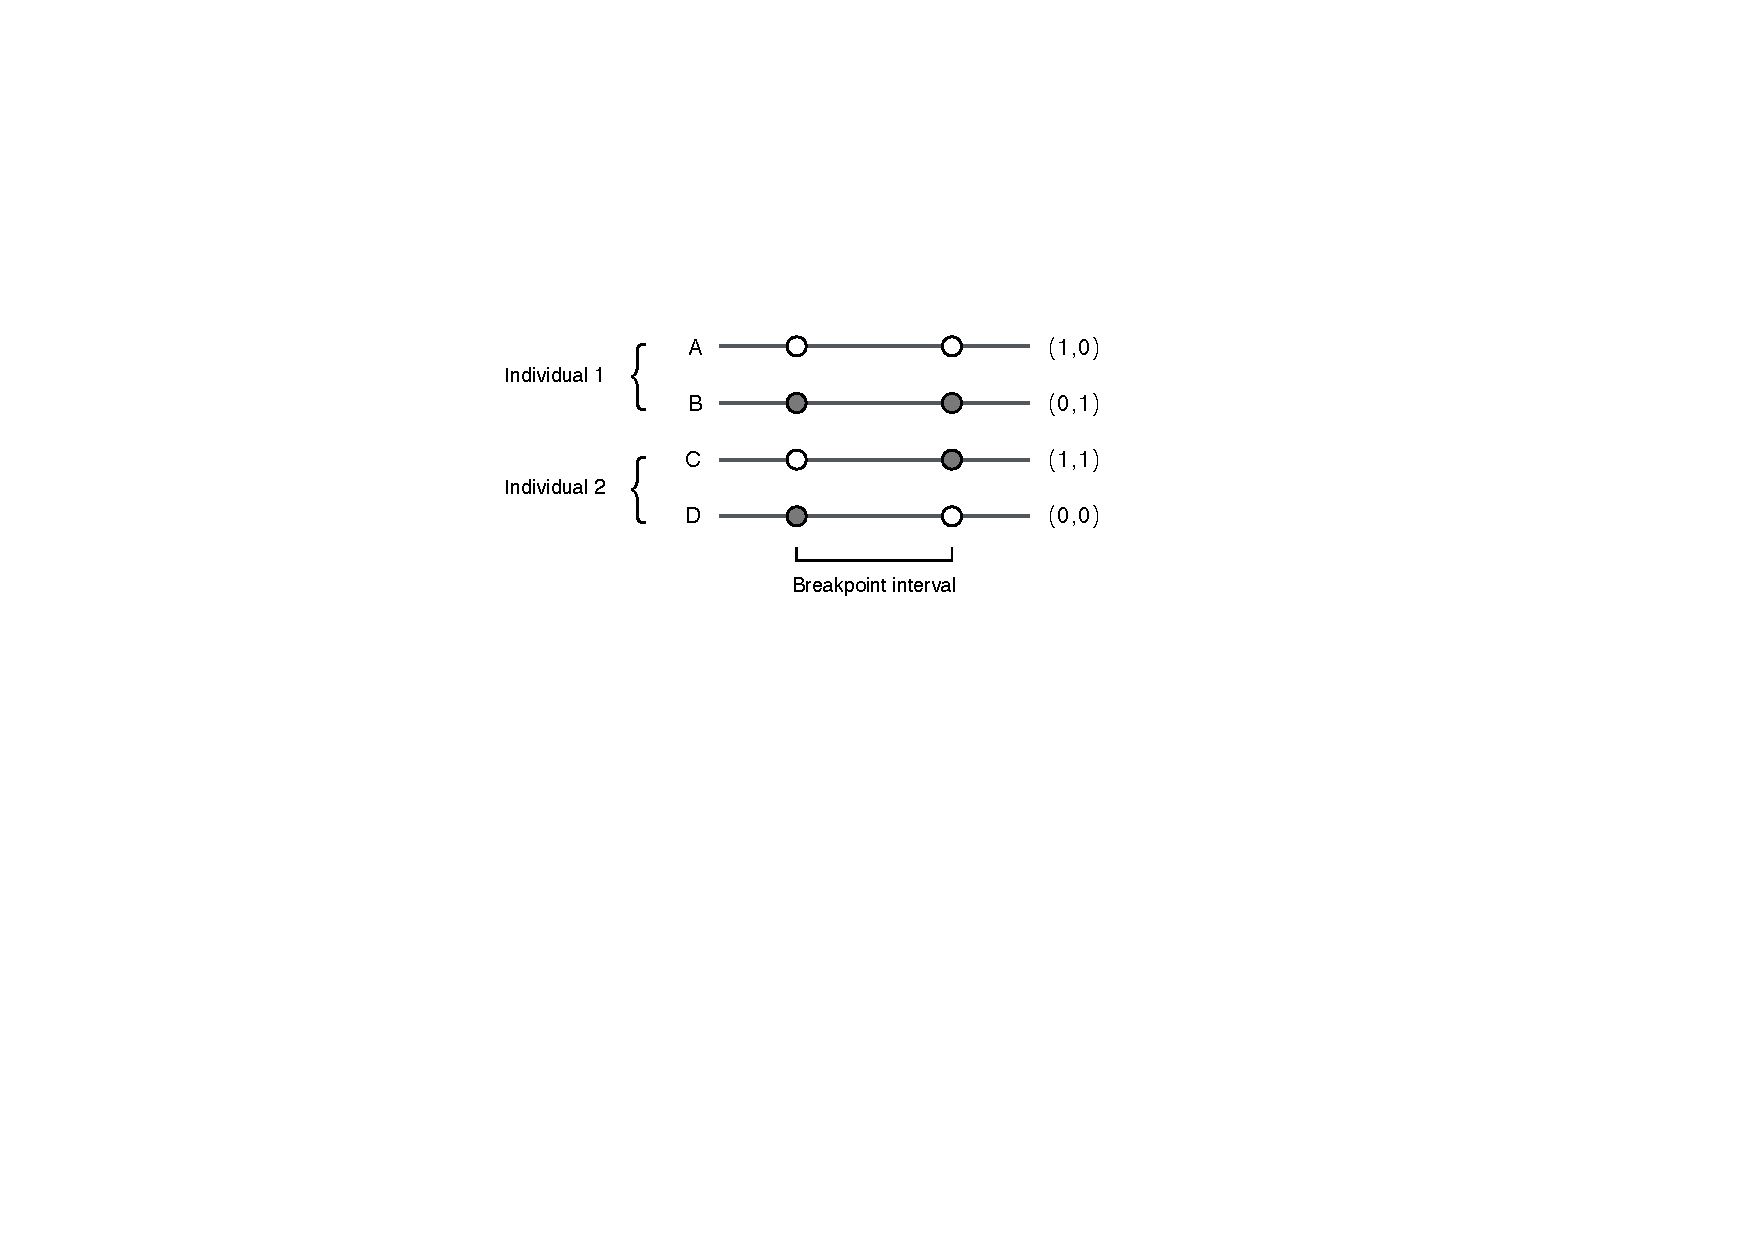
\includegraphics[width=0.7\textwidth]{./img/ch3/info_fgt}
\Caption{Breakpoint detection using the four-gamete test (FGT)}
{The \n{4} haplotypes (gametes) in a pair of \n{2} diploid individuals are shown (\emph{horizontal lines}).
A breakpoint interval is detected if all \n{4} possible allelic state configurations are observed at \n{2} variant sites along the sequence.
The interval delimits the region in which at least \n{1} recombination event must have occurred in the history of the sample (given the assumptions of the infinite sites model).
The \n{4} allelic state configurations are shown on the \emph{right}.
The alleles are shown at the \n{2} breakpoint sites; indicated as ancestral (\emph{hollow} circle) and derived state (\emph{solid}).
Note that the order of gametes is ignored.}
{fig:info_fgt}
\end{figure}

%

Notably, private or \emph{de~novo} mutations appearing as singletons in the sample cannot lead to the observation of the \n{4} required configurations.
Although the exact location of chromosomal crossover cannot be retrieved from the data, the \gls{fgt} can be used to find the smallest interval in which recombination occurred.
\Addition{However, it is important to note that this test cannot determine which of the four haplotypes recombined, and where it is also possible that there have been multiple recombination events between any two of the four haplotypes within the detected interval.
Also, while it would be possible to consider other individuals to infer recombination events that have occurred in the sample, the purpose of this implementation is to detect recombination between haplotypes contained within two individuals sharing a given focal allele.}


\paragraph{\Gls{dgt}.}
In absence of haplotype information, data are represented as genotypes, where genotypic states are encoded as 0, 1, and 2, for variants that are homozygous for the ancestral allele, heterozygous, and homozygous for the derived allele, respectively.
Given the genotype sequences of \n{2} diploid individuals, recombination is inferred between \n{2} sites; one being heterozygous in both individuals (\ie the genotypes 1 and 1) and another with opposite homozygous genotypes (0 and 2).
In the latter case, it follows that the \n{2} individuals cannot share a haplotype at that locus.

The \gls{dgt} is a special case of the \gls{fgt}, as the same composition of alleles is implied.
For example, if the allelic configurations ${(0,1)}$ and ${(0,0)}$ are seen in individual~1, and configurations ${(1,0)}$ and ${(1,1)}$ in individual~2, the corresponding genotypic configurations are ${(0,1)}$ and ${(2,1)}$, respectively, which satisfies the breakpoint condition in both the \gls{fgt} and \gls{dgt}.
However, because genotype data result from haplotype occurrence in individuals, not all breakpoints detectable under the \gls{fgt} can be found using the \gls{dgt}.
At sites where the \gls{fgt} detects a breakpoint interval, the \gls{dgt} cannot break if both sites are heterozygous in the same individual.
As a consequence, it can be expected that the \gls{dgt} is more restrictive than the \gls{fgt}; \eg if breakpoints are found, they are likely to sit farther apart.

%
%!TEX root = ../../main.tex


\begin{figure}[!htb]
\centering
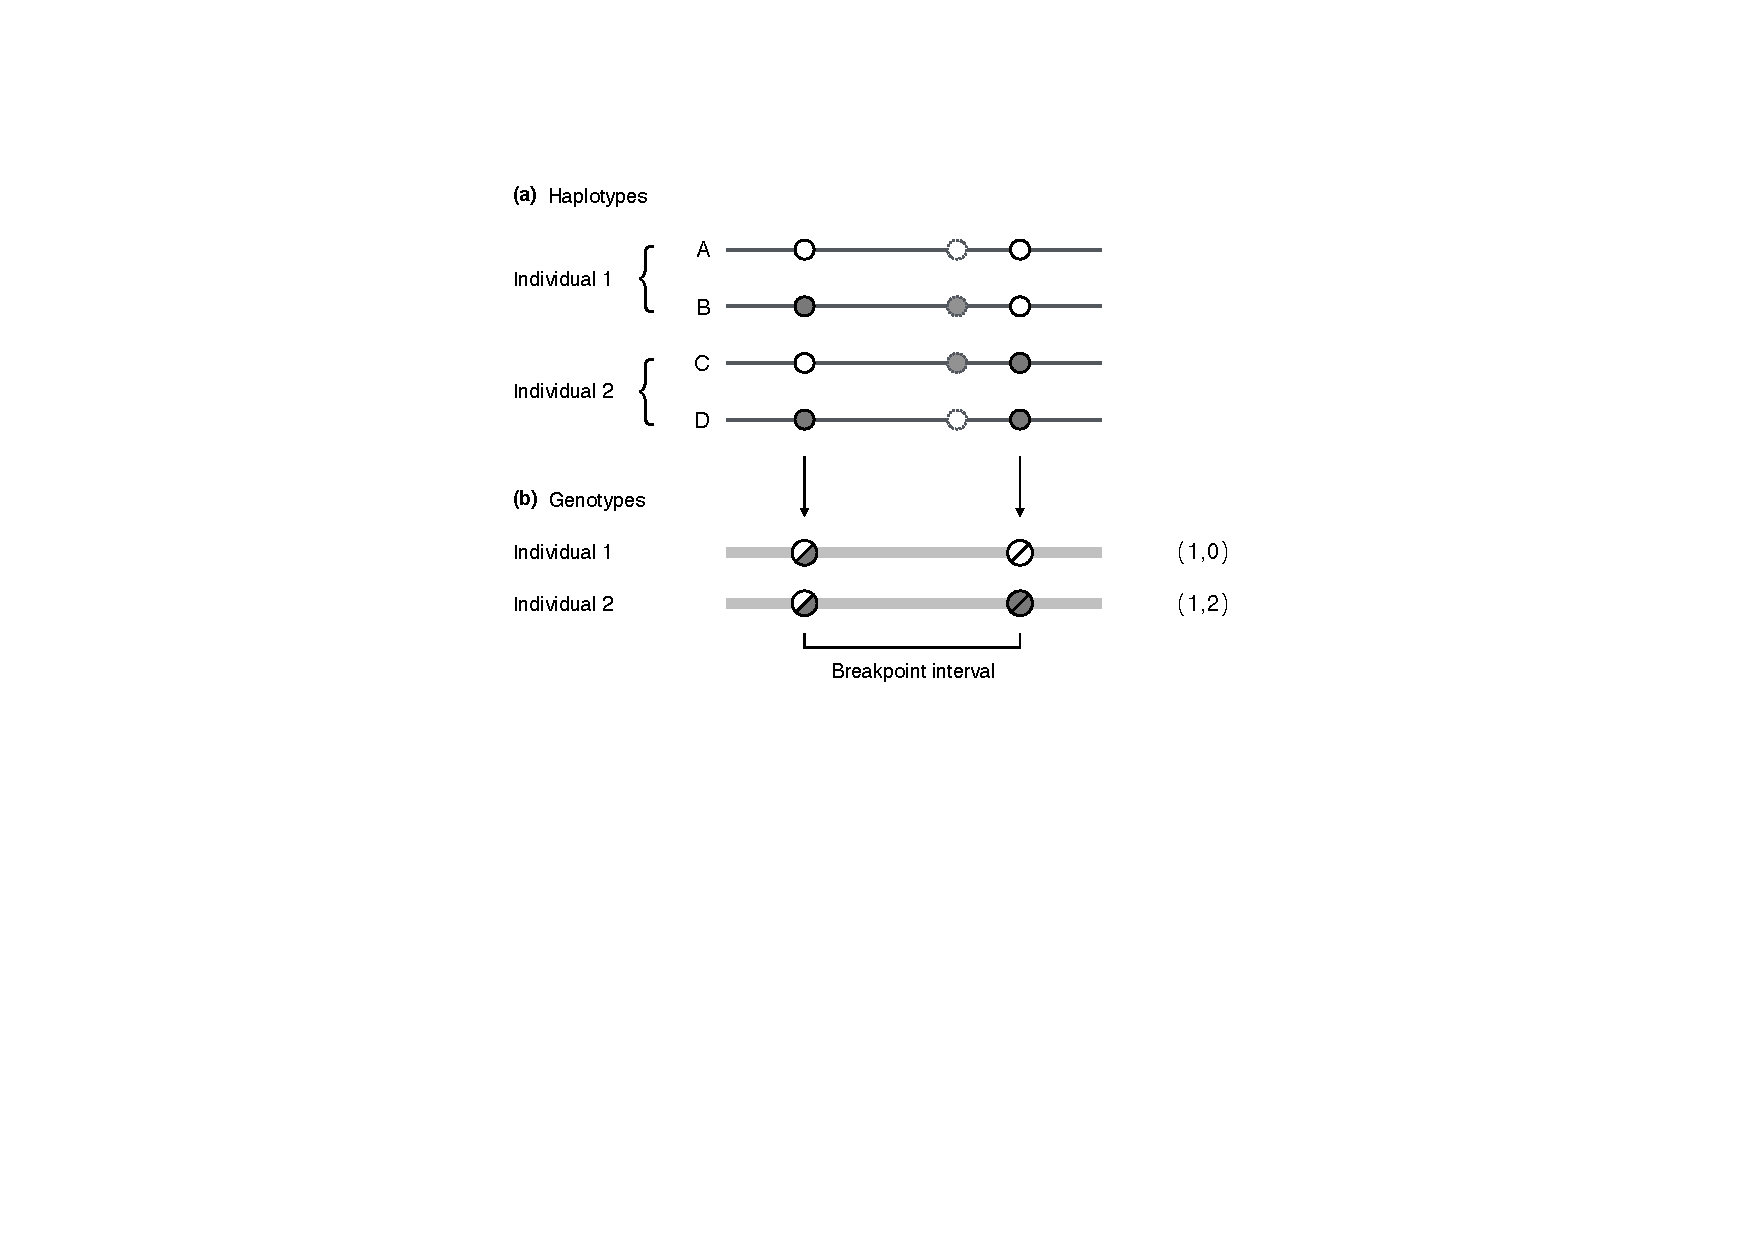
\includegraphics[width=0.7\textwidth]{./img/ch3/info_dgt}
\Caption{Breakpoint detection using the discordant genotype test (DGT)}
{Unlike the \gls{fgt}, which requires haplotype information, the \gls{dgt} identifies a breakpoint interval using genotype data.
For comparison, Panel~\textbf{(a)} shows the \n{4} gametes of the \n{2} individuals involved; see \cpref{fig:info_fgt}.
To highlight the difference to the \gls{fgt}, an additional variant is shown in between both sites; alleles indicated by a \emph{dotted} edge.
This site would satisfy the breakpoint condition under the \gls{fgt}, but is missed under the \gls{dgt}.
Panel~\textbf{(b)} shows the \n{2} genotype sequences per individual (\emph{thick} horizontal lines) from which a breakpoint interval is inferred using the \gls{dgt}.
The genotypic states of the breakpoint sites are given on the \emph{right}.
Genotypes can either be homozygous for the ancestral allele (\emph{hollow} circle), heterozygous (\emph{semi-solid}), or homozygous for the derived allele (\emph{solid}).}
{fig:info_dgt}
\end{figure}

%

\Addition{The \gls{dgt} thereby simplifies the breakpoint condition to observing opposite homozygote genotypes in two diploid individuals, but where allele sharing at a given target site (that is heterozygous in both individuals) is required such that the conditions of the \gls{fgt} would be satisfied.}
This is further exemplified in \cpref{fig:info_dgt}, which highlights the difference to the \gls{fgt} by comparison to the example shown in \cpref{fig:info_fgt}.


%
\subsection{Description of the algorithm}
%

The \gls{fgt} and \gls{dgt} provide the means for non-probabilistic inference of recombination breakpoints from either haplotype or genotype data, respectively.
This methodology is implemented such that the full length of an IBD segment can be found around a given target site in a pair of diploid individuals.
The allele at a target site serves as an indicator for haplotype sharing by descent; hence, to detect recent IBD, rare variants are used as primary targets.
The aim of this method is to infer breakpoint intervals independently on both sides of the target position along the sequence, so as to infer the \n{2} recombination events that delimit the underlying IBD segment.
As such, the target variant is set as the \emph{focal} breakpoint.
The algorithm is described below; a more intuitive example is illustrated in \cpref{fig:info_breakpoint}.

%
%!TEX root = ../../main.tex


\begin{figure}[!tbp]
\centering
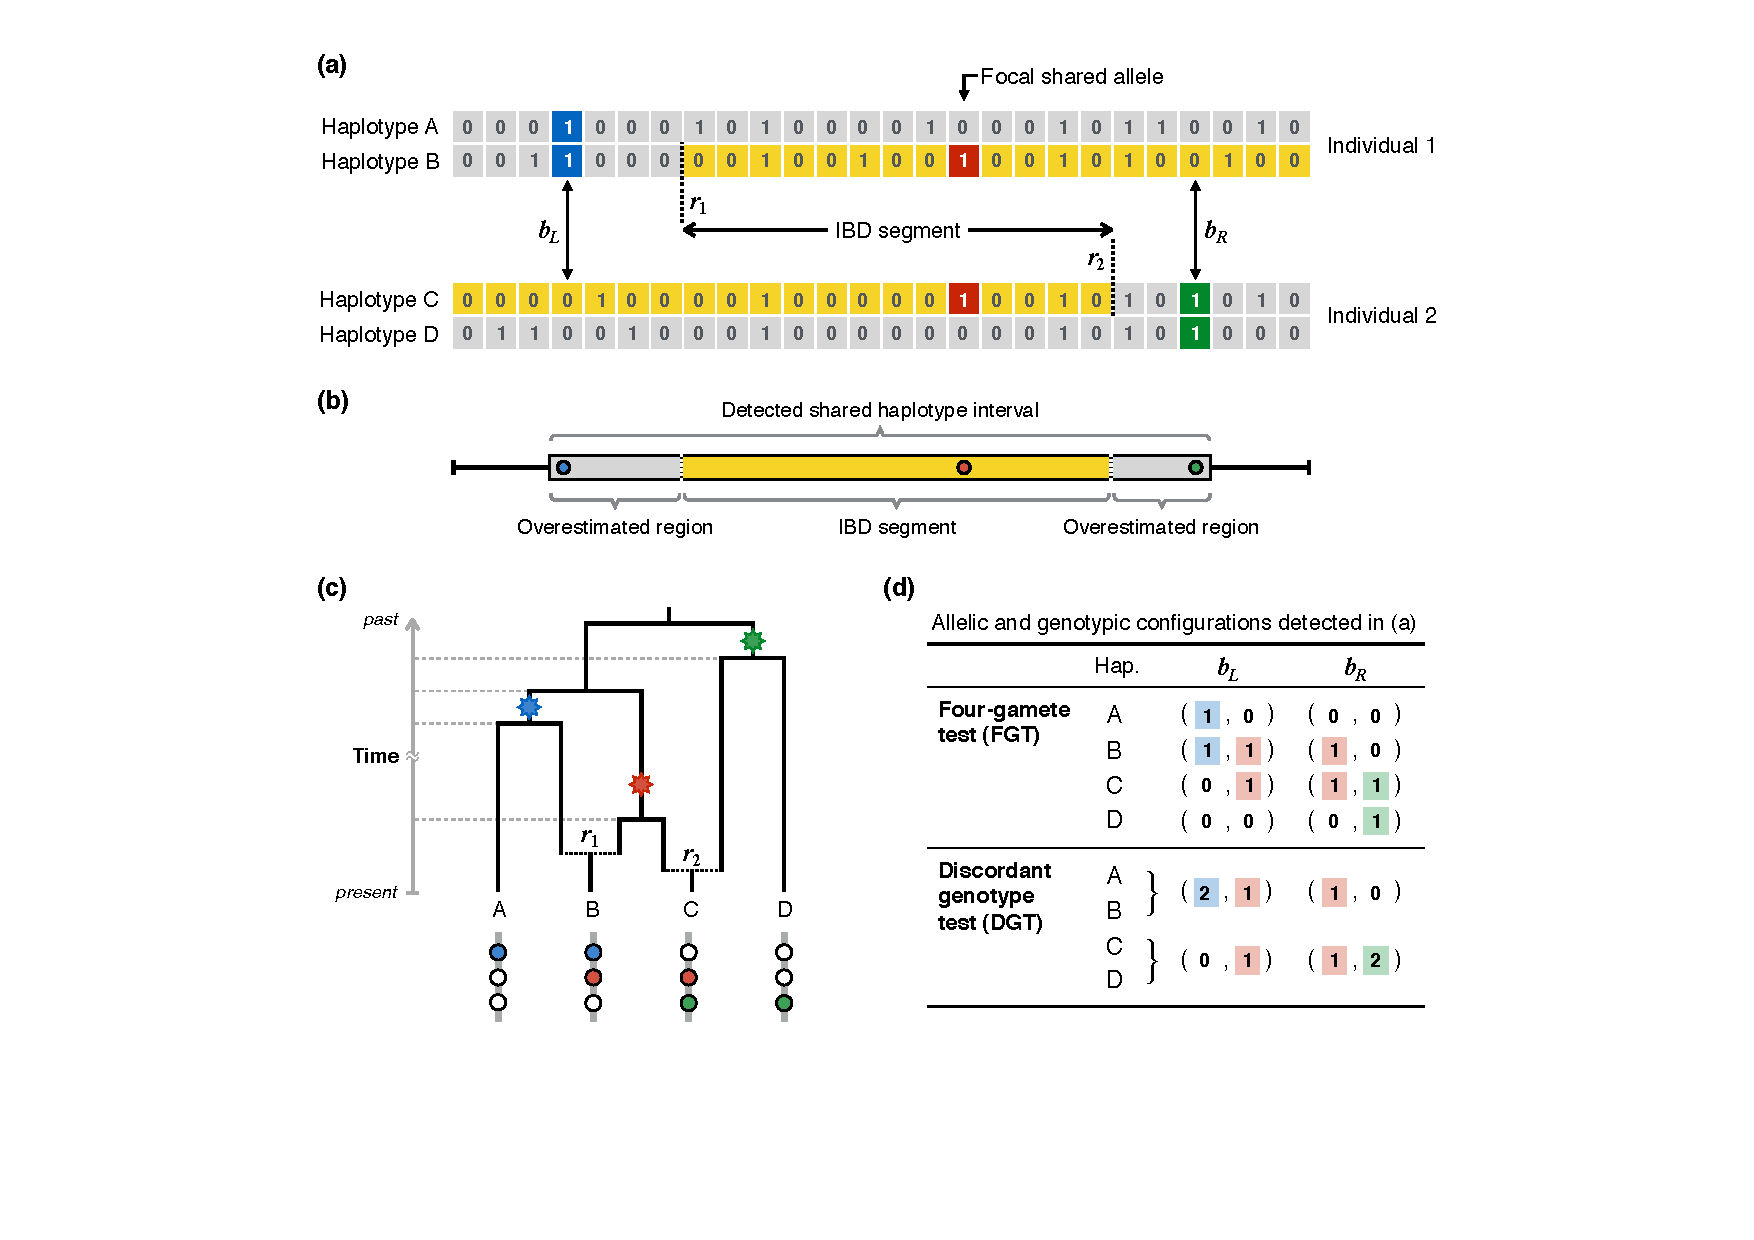
\includegraphics[width=\textwidth]{./img/ch3/info_breakpoint}
\Caption{Illustration of shared haplotype detection in a pair of diploid individuals}
{Panel~\textbf{(a)} shows \n{2} individuals composed of haplotypes A and B, and haplotypes C and D, respectively.
Each haplotype is represented as a sequence of observed allelic states, where $0$ and $1$ denote the ancestral and derived allele, respectively.
Breakpoints are detected by independently scanning to the left and right-hand side from the target position.
The \n{2} individuals share a haplotype by descent (highlighted in \emph{yellow}) which is tagged by the focal allele (\emph{red}), for which the \n{2} individuals are heterozygous
\N{2} sites (\emph{blue} and \emph{green}) mark the first sites at which a breakpoint condition is satisfied, such that $b_{L}$ and $b_{R}$ are detected.
The IBD segment shared by both individuals is indicated by $r_{1}$ and $r_{2}$ (\emph{dashed lines}).
Panel~\textbf{(b)} shows the detected breakpoint interval, delimited by $b_{L}$ and $b_{R}$ (inclusive).
Note that detected breakpoints are only the first indication of recombination found distal to the focal site, but may not mark the points of the actual crossover events; thus, it is expected that the length of the detected segment is overestimated, dependent on available data.
Panel~\textbf{(c)} represents the history of the sample as an \gls{arg}.
Mutation events are indicated on the tree (\emph{stars}) and gave rise to the alleles highlighted in~(a); \emph{blue}, \emph{red}, and \emph{green}.
The dotted \emph{grey} lines indicate the time of coalescent events in the history of the sample; dotted \emph{black} lines indicate recombination events.
Panel~\textbf{(d)} provides a table outlining the configurations of allelic and genotypic states at breakpoint sites as considered in the \gls{fgt} and \gls{dgt}, respectively.
Notably, in the example shown, both the \gls{fgt} and \gls{dgt} detect breakpoints at indicated sites.
But, for example, if individual~1 was composed of haplotypes A and C, and individual~2 of haplotypes B and D, the breakpoints would be detected as shown under the \gls{fgt}, but not the \gls{dgt}.}
{fig:info_breakpoint}
\end{figure}

%

Let $M$ be the number of variant sites observed in a sample of $N$ diploid individuals.
At the target site, $b_{i}$, where ${i \in \lbrace 1, 2, \ldots, M \rbrace}$, the subset of individuals sharing the derived allele is identified and compared in a pairwise fashion.
Importantly, the allele at this site is used as an identifier for haplotype sharing, on which inference is conditioned in either the \gls{fgt} or \gls{dgt}.
Thus, individuals are only considered if they are heterozygous for the focal allele, as the breakpoint condition in either test cannot be satisfied otherwise.
However, note that this restriction arises from the variant-centric focus on a given rare allele; \eg the condition of the \gls{fgt} could be satisfied for individuals homozygous for a given allele, but without that the allele is shared by the other individual (hence, defying the purpose of this implementation).
In each pair, chromosomes are scanned to the left and right-hand side from the target site until the first site is found that, together with the allelic or genotypic states observed at $b_{i}$, satisfies the breakpoint condition, which is done independently on each side.
Detected breakpoints are labelled as $b_{L}$ and $b_{R}$ on the left and right-hand side, respectively, such that the intervals ${[b_{L}, b_{i}]}$ and ${[b_{i}, b_{R}]}$ delimit the chromosomal regions in which recombination events occurred, respectively; where ${L,R \in \lbrace 1, 2, \ldots, M \rbrace}$.
Hence, the underlying IBD segment is enclosed in ${[b_{L}, b_{R}]}$.

The allelic or genotypic states at $b_{L}$ or $b_{R}$ provide only the first indication of recombination found along the sequence on either side of the focal allele, but may not mark the points of the actual crossover events.
The detected interval is therefore inclusive of the breakpoints such that the full length of the underlying IBD segment is covered.
%However, this is expected to lead to an overestimation of the shared haplotype length.
In cases where the end of a chromosome is reached without detecting any evidence of recombination, the terminal site is recorded to capture the length of the segment; this is hereafter referred to as a \emph{boundary case}.

%%%%%%%%%%%%%%%%%%%%%%%%%%%%%%%%%%%%%%%%%%%%%%%%%%%%%%%%%%%%%%%%%%%%%%%%%%%%%%

Note that a recombination event can occur with chromosomes outside the sub-tree of the lineages deriving from the focal mutation, such that a breakpoint may be falsely inferred.
Consider individual~1 with haplotypes ${\{A,B\}}$ and individual~2 with haplotypes ${\{C,D\}}$, where haplotypes $B$~and~$C$ share a focal allele at a given site such that their lineages form a sub-tree.
The IBD segment between $B$~and~$C$ is delimited by the two nearest recombination events on either side, but where it is possible that either $A$~and~$B$ or $C$~and~$D$
Breakpoints are eventually found by independently scanning to the left and right-hand side, either using the \gls{fgt} or \gls{dgt}, but where it cannot be known which pair of haplotypes (among the four contained within the two individuals) recombined.
It is possible, for example, that
however, such cases are assumed to be sufficiently rare and treated as being negligible.

%%%%%%%%%%%%%%%%%%%%%%%%%%%%%%%%%%%%%%%%%%%%%%%%%%%%%%%%%%%%%%%%%%%%%%%%%%%%%%


%
\subsection{Anticipated limitations}
%

As noted by \citet{Hudson:1985wh}, not all recombination events in the history of a sample are found by the \gls{fgt}, and are therefore also missed by the \gls{dgt}.
In the implementation presented, a breakpoint is found by performing a scan along the sequence away from a target position.
Provided that the neighbouring haplotype regions derive from different ancestral lineages, in the general case, it is likely that a breakpoint will be found eventually (or the boundary of the chromosome is reached).

The main limitation to the accuracy of the detected breakpoints is the overestimation of the interval, in relation to the underlying true IBD length; as shown in \cref{fig:info_breakpoint}{b}.
While the underlying IBD segment is enclosed in the interval, it can be expected that breakpoints are detected at sites some distance away from where recombination occurred, thus overestimating the true length of the underlying IBD tract.
The extent of overestimation is dependent on the number and density of observed variant sites in the sample.
This suggests that the method may become more accurate with larger samples\Addition{, as the number of segregating sites observed in the sample is expected to increase with sample size}.
Likewise, because the rate of mutation is directly proportional to the expected number of segregating sites \citep{Watterson:1975ur}, a higher mutation rate can generally be expected to decrease the overestimation of segment length.

%
%!TEX root = ../../main.tex


\begin{figure}[!htbp]
	% {\scriptsize \texthv{\textbf{(a)} Example 1}} \\
	% 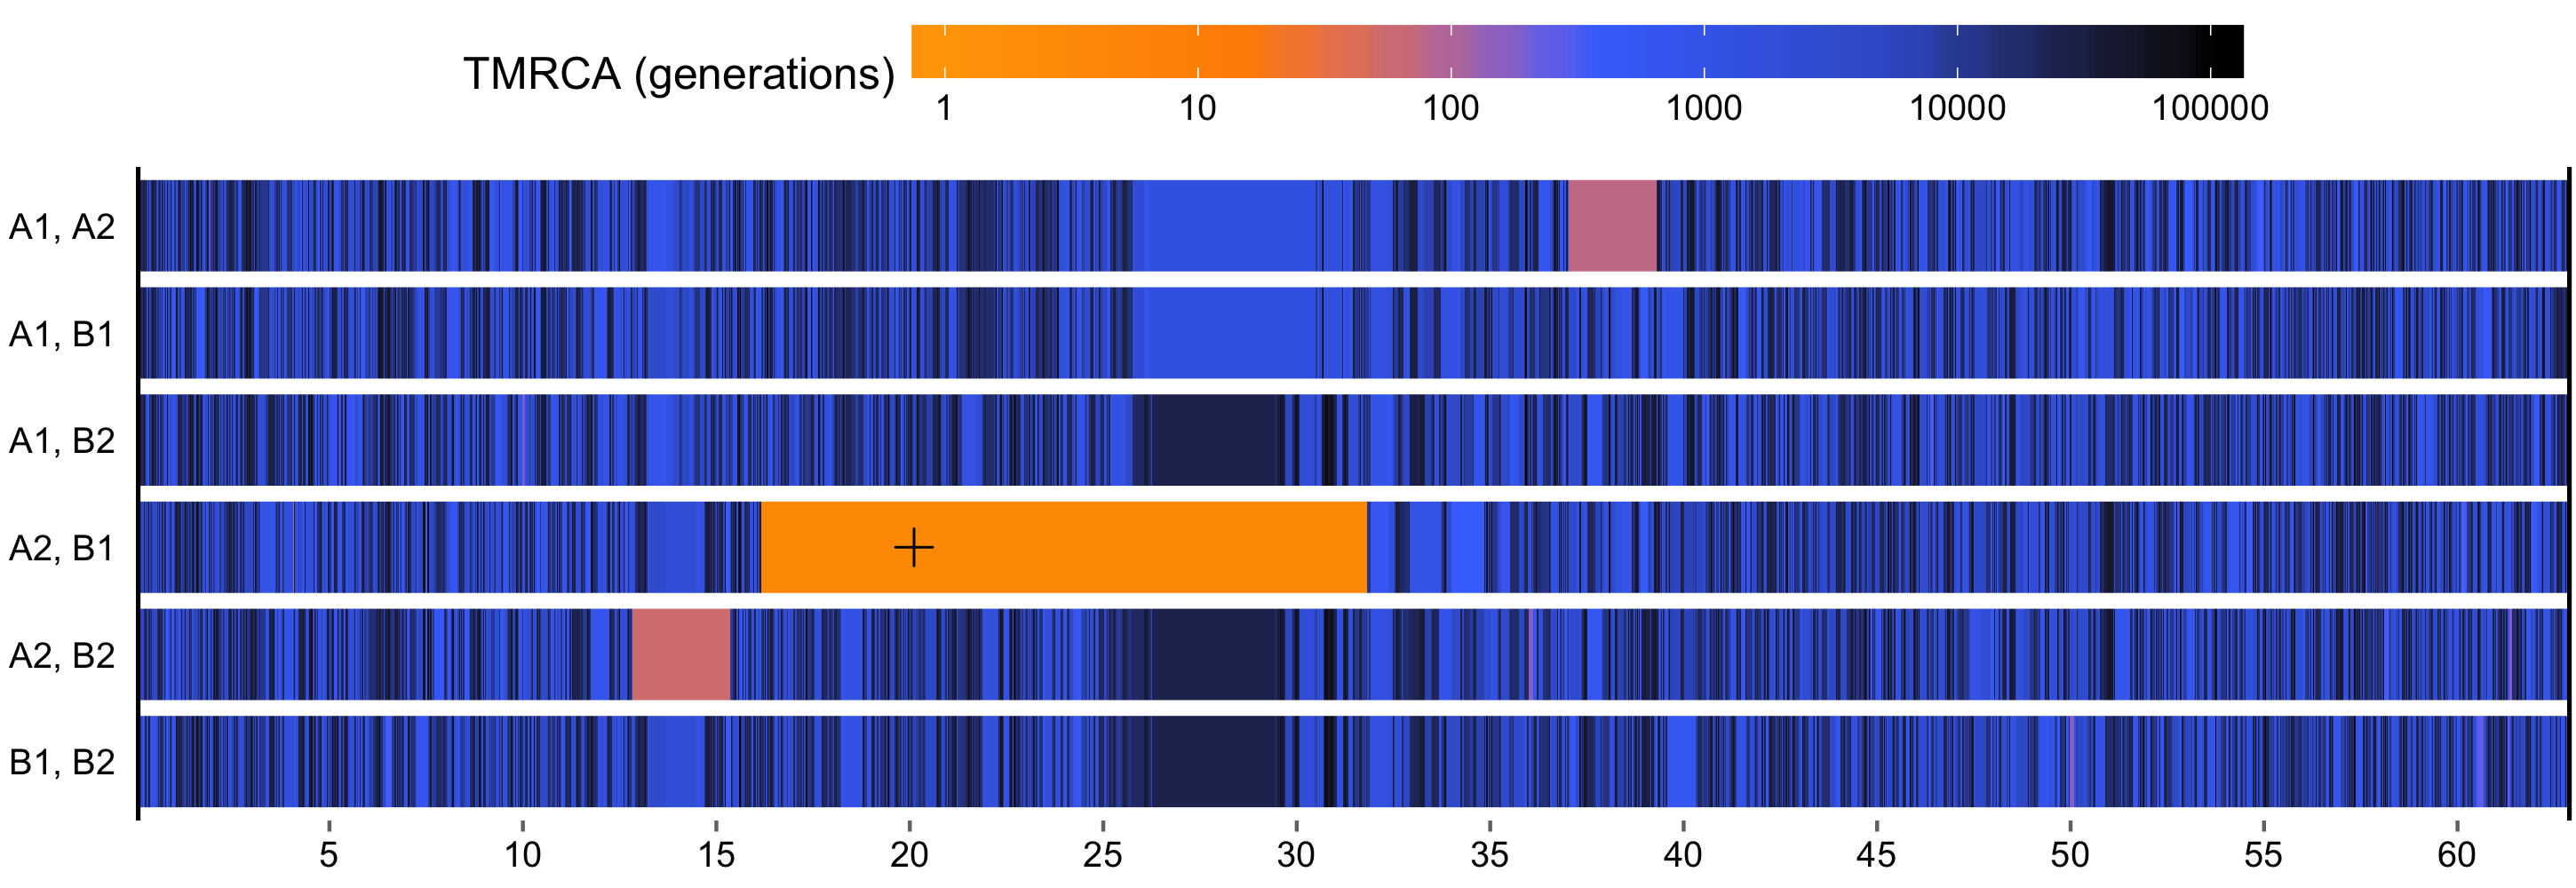
\includegraphics[width=\textwidth]{./img/ch3/full_ibd_example_A.png}
	% 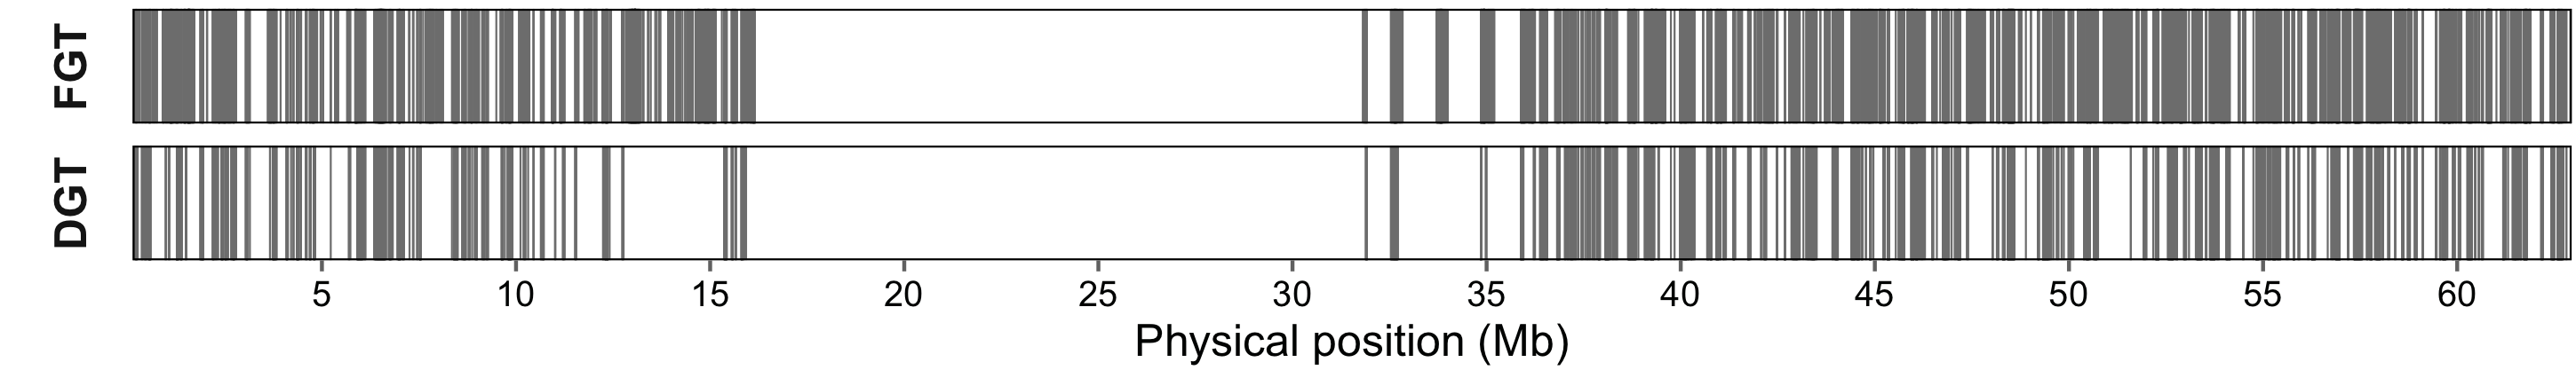
\includegraphics[width=\textwidth]{./img/ch3/full_ibd_example_B.png}
	% {\scriptsize \texthv{\textbf{(b)} Example 2}} \\
	% 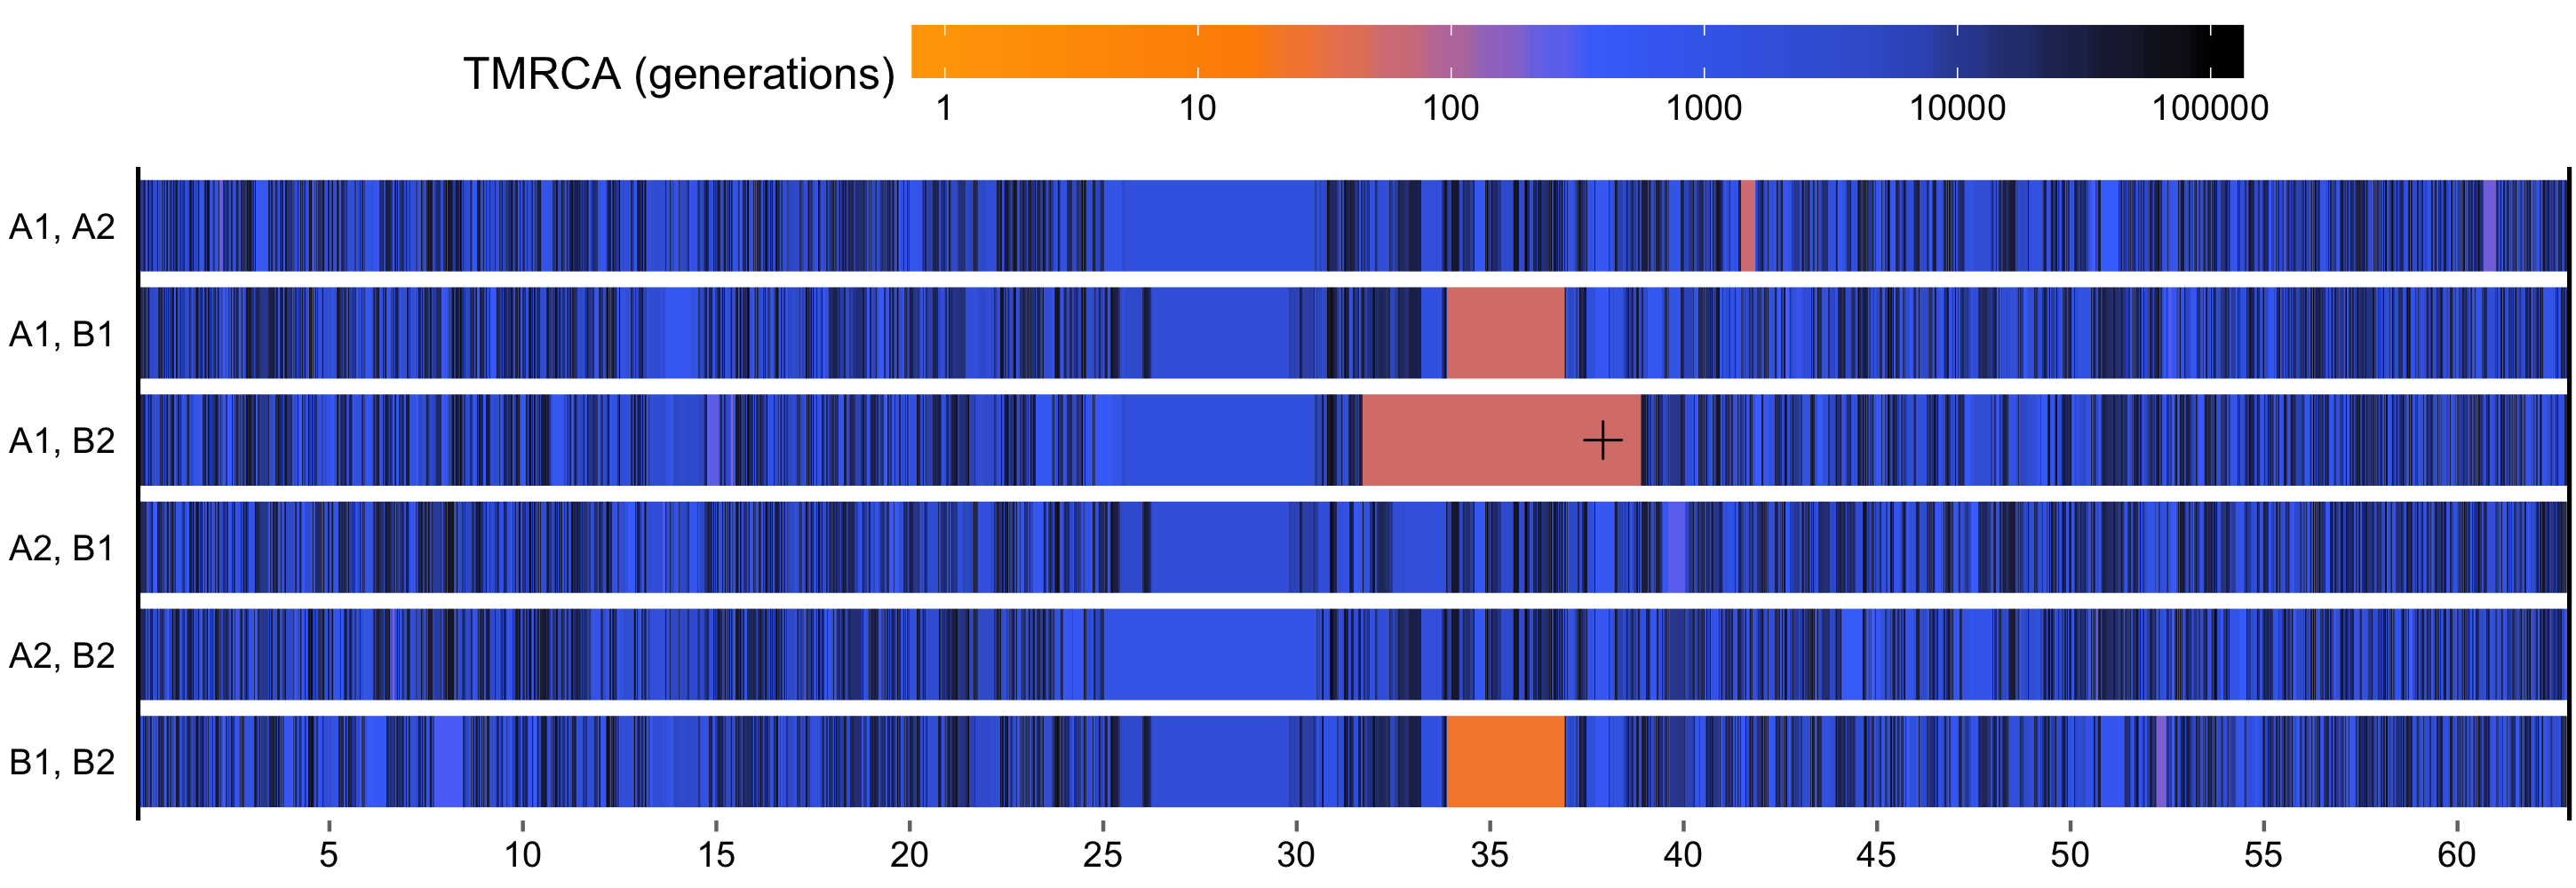
\includegraphics[width=\textwidth]{./img/ch3/full_ibd_underest_A.png}
	% 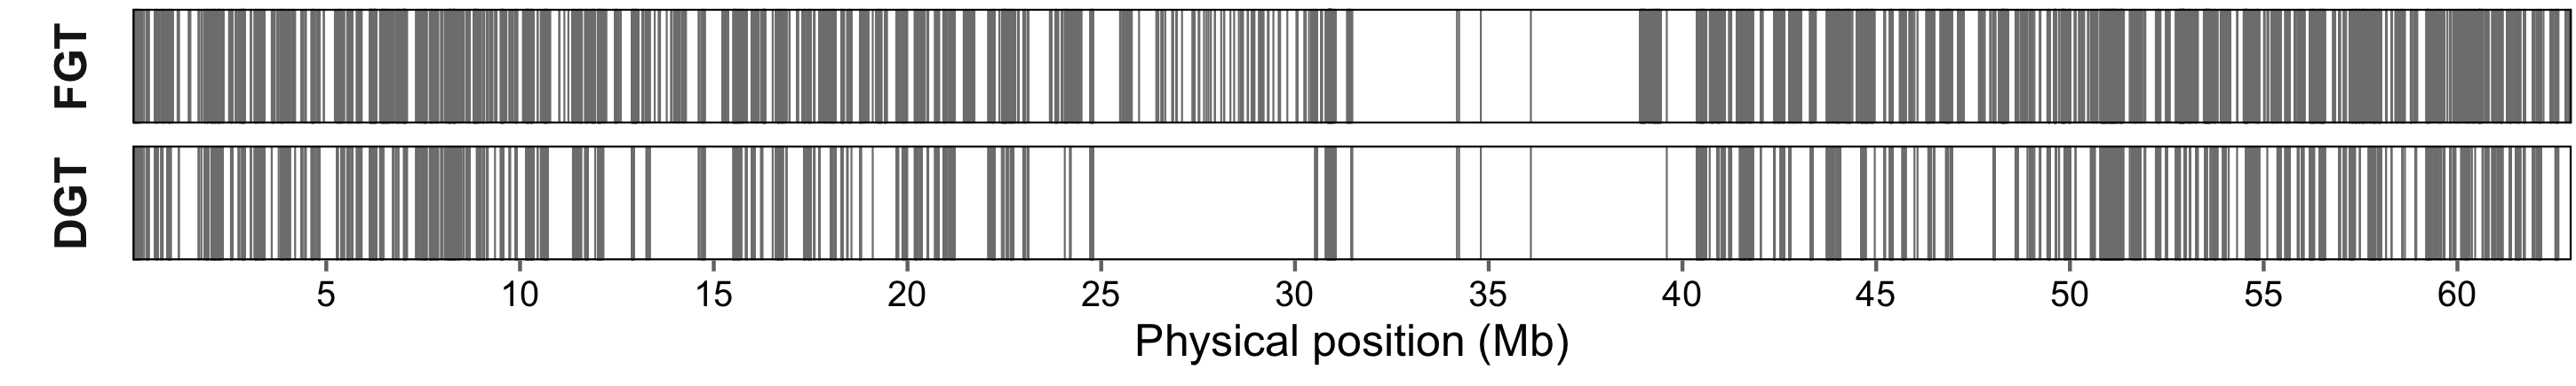
\includegraphics[width=\textwidth]{./img/ch3/full_ibd_underest_B.png}
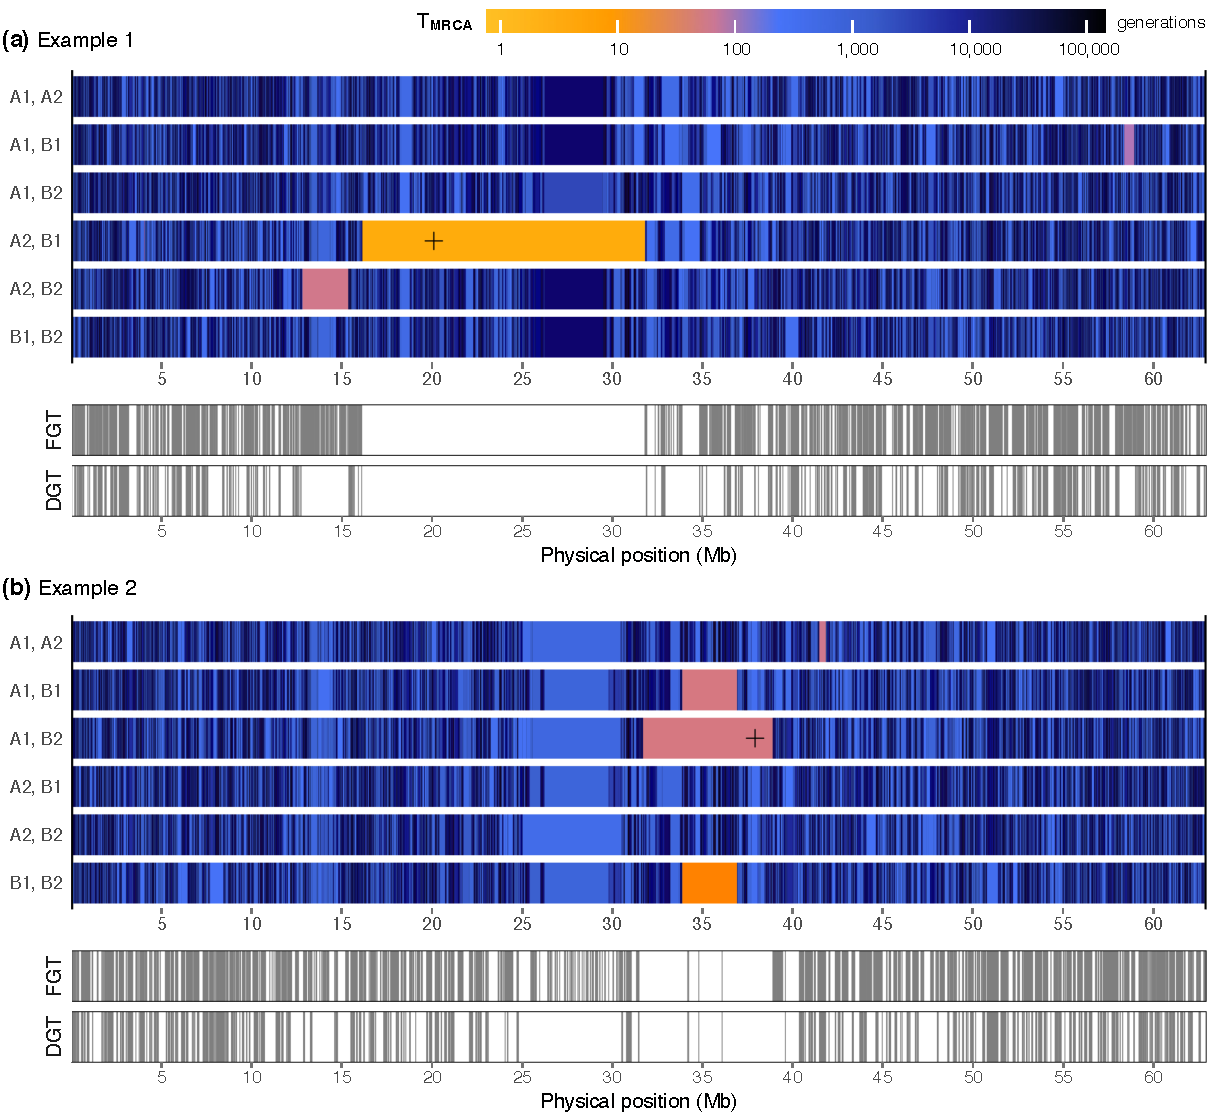
\includegraphics[width=\textwidth]{./img/ch3/full_ibd_example}
\Caption{Examples of the underlying IBD structure in each pair of four chromosomes}
{The true, underlying IBD structure is shown for each possible pair among \n{4} chromosomes in \n{2} diploid individuals; \n{2} examples are shown.
Each chromosome is labelled by its occurrence in individuals A~and~B, where chromosomes~1~and~2 are distinguished.
The ``mosaic'' of IBD segments per pair was determined from coalescent records produced in simulations using \texttt{msprime} \citep{Kelleher:2016fn}; see \cpref{sec:msprime}.
Each segment defines the region that was co-inherited from a \gls{mrca}, and is colour-coded by the number of generations separating the \n{2} chromosomes from their shared \gls{mrca} in that region.
The \emph{cross} marks the position of the focal allele in the pair that shares it.
Below, all breakpoints detected relative to the focal variant along the simulated region are indicated, using the \gls{fgt} (\emph{top}) and \gls{dgt} (\emph{bottom}).
Panel~\textbf{(a)} shows that the innermost breakpoint intervals (relative to the target position) detected in the \gls{fgt} or \gls{dgt} align closely with the true termini of the IBD segment.
The extent of overestimation appears to be negligible in relation to the length of the detected segment.
Panel~\textbf{(b)} shows that the innermost intervals are underestimated, due to an overlap of recently co-inherited haplotypes on different chromosome pairs.}
{fig:full_ibd_example}
\end{figure}

%

Conversely, it is also possible that segment length is underestimated.
Given the \n{4} chromosomes required, there are ${{{4}\choose{2}}=6}$ possible pairs of chromosomes which may share extended regions by descent.
For example, if \n{2} individuals share multiple IBD tracts at different pairs of their chromosomes, these tracts may overlap.
In such cases, breakpoint detection cannot distinguish between overlapping segments.
This is illustrated in \cpref{fig:full_ibd_example}, which shows \n{2} examples generated using coalescent simulations.

In Example~1 (\ref{fig:full_ibd_example}{a}), a rare allele target site was randomly selected, as well as the \n{2} individuals sharing the this allele.
The true IBD structure was determined from simulation records for each pair of the \n{4} chromosomes in the \n{2} individuals.
Each pair is represented by a mosaic of IBD segments along the sequence, where each segment is distinguished by \gls{tmrca}.
Both the \gls{fgt} and \gls{dgt} were applied, but where all consecutive breakpoints after the first detection were also recorded along the sequence on both sides of the focal variant.
The innermost interval delimits the detected shared haplotype segment around the target site.
Example~1 illustrates the general case in which a rare allele identifies the underlying co-inherited haplotype segment, which may stand out as being much younger due to recent shared ancestry.

The same was done in Example~2 (\ref{fig:full_ibd_example}{b}), but here the target site and the pair of individuals was chosen because it was found that the length of the detected IBD segment was underestimated.
As can be seen, this underestimation is due to an overlap of multiple pairwise shared IBD tracts in other chromosome pairs within the same pair of individuals.
Such a result may be expected in cases of inbreeding, where the maternal and paternal chromosomes in an individual are more closely related to each other than to other chromosomes in the population.
Note that in the simulations conducted, the generated haplotypes were randomly paired to form diploid individuals.



\DeleteNote{Section ``Genotype phasing by inference of the shared haplotype''}
%
% %
% \section{Genotype phasing by inference of the shared haplotype}
% \label{sec:ibd_phasing}
% %
%
% In this section, I extend the IBD detection method such that the allelic sequence of the shared haplotype can be deduced.
% Since it is assumed that a breakpoint interval covers a region in which \n{2} individuals share a haplotype recently co-inherited from a common ancestor, in principle it is possible to infer the shared haplotype sequence based on genealogical constraints.
% By knowing the sequence of the shared haplotype, it follows that the sequences of the ``unshared'' haplotypes in both individuals can be derived.
% The approach presented can therefore be seen as an application to genotype \emph{phasing}, \ie the inference of haplotypes from genotype data, which has become a fundamental problem in genetic research \citep{Browning:2011ic}.
%
% Currently, the most accurate and widely employed phasing algorithms are designed to infer haplotype sharing using \glspl{hmm}, which typically operate under a probabilistic model of coalescence with recombination \citep{Stephens:2001kh,Delaneau:2008dk}.
% Notable examples include computational tools such as \texttt{SHAPEIT} \citep{Delaneau:2011iu,Delaneau:2013hi} and \texttt{EAGLE} \citep{loh2016fast,Loh:2016bl}.
% The basic phasing process can be described in context of the influential \citet{Li:2003uz} model, where haplotypes are reconstructed from genotype data as ``imperfect mosaics'' of other haplotypes (\eg using a reference panel).
% Existing phasing methods typically show high levels of accuracy.
% However, the phase at low-frequency variants is often problematic to resolve because patterns of allelic variation or \gls{ld} may be too rare to allow correlation with available haplotype information.
%
% Here, I explore the feasibility of phasing genotypes at sites within a given breakpoint interval using the IBD detection method presented in the previous section; haplotypes are therefore inferred \emph{locally} and are limited to the region covered by the interval.
% In the following, I explain the genealogical constraints that determine the possible haplotype allocation of alleles in genotype data.
% I then describe the general phasing approach as implemented here.
%
% %
% \subsection{Genealogical constraints arising from IBD}
% %
%
% At a given site, the genotypic states observed at \n{2} diploid individuals represent the sum of alleles, where each allele derives from a mutation event on some branch of the genealogical tree of the sample.
% By knowing that \n{2} haplotypes were co-inherited from a recent \gls{mrca}, a part of this unseen genealogy is resolved, such that certain genotypes can only be formed if mutation events occurred on certain branches of the tree.
% This can be seen as being analogous to having partial pedigree information; \ie the \n{2} individuals are implicitly treated as the ``offspring'' of their ancestral ``parent''.
% By following the line of descent, the ancestral haplotype can be inferred if consistent with observed genotypes.
% However, here, the assumed pedigree is incomplete, because ancestral relations of the \n{2} unshared haplotypes are not known from available IBD information.
% There is nonetheless sufficient information to deduce the allelic states given certain genotypic arrangements.
%
% %
% %!TEX root = ../../main.tex


\begin{figure}[!htb]
\centering
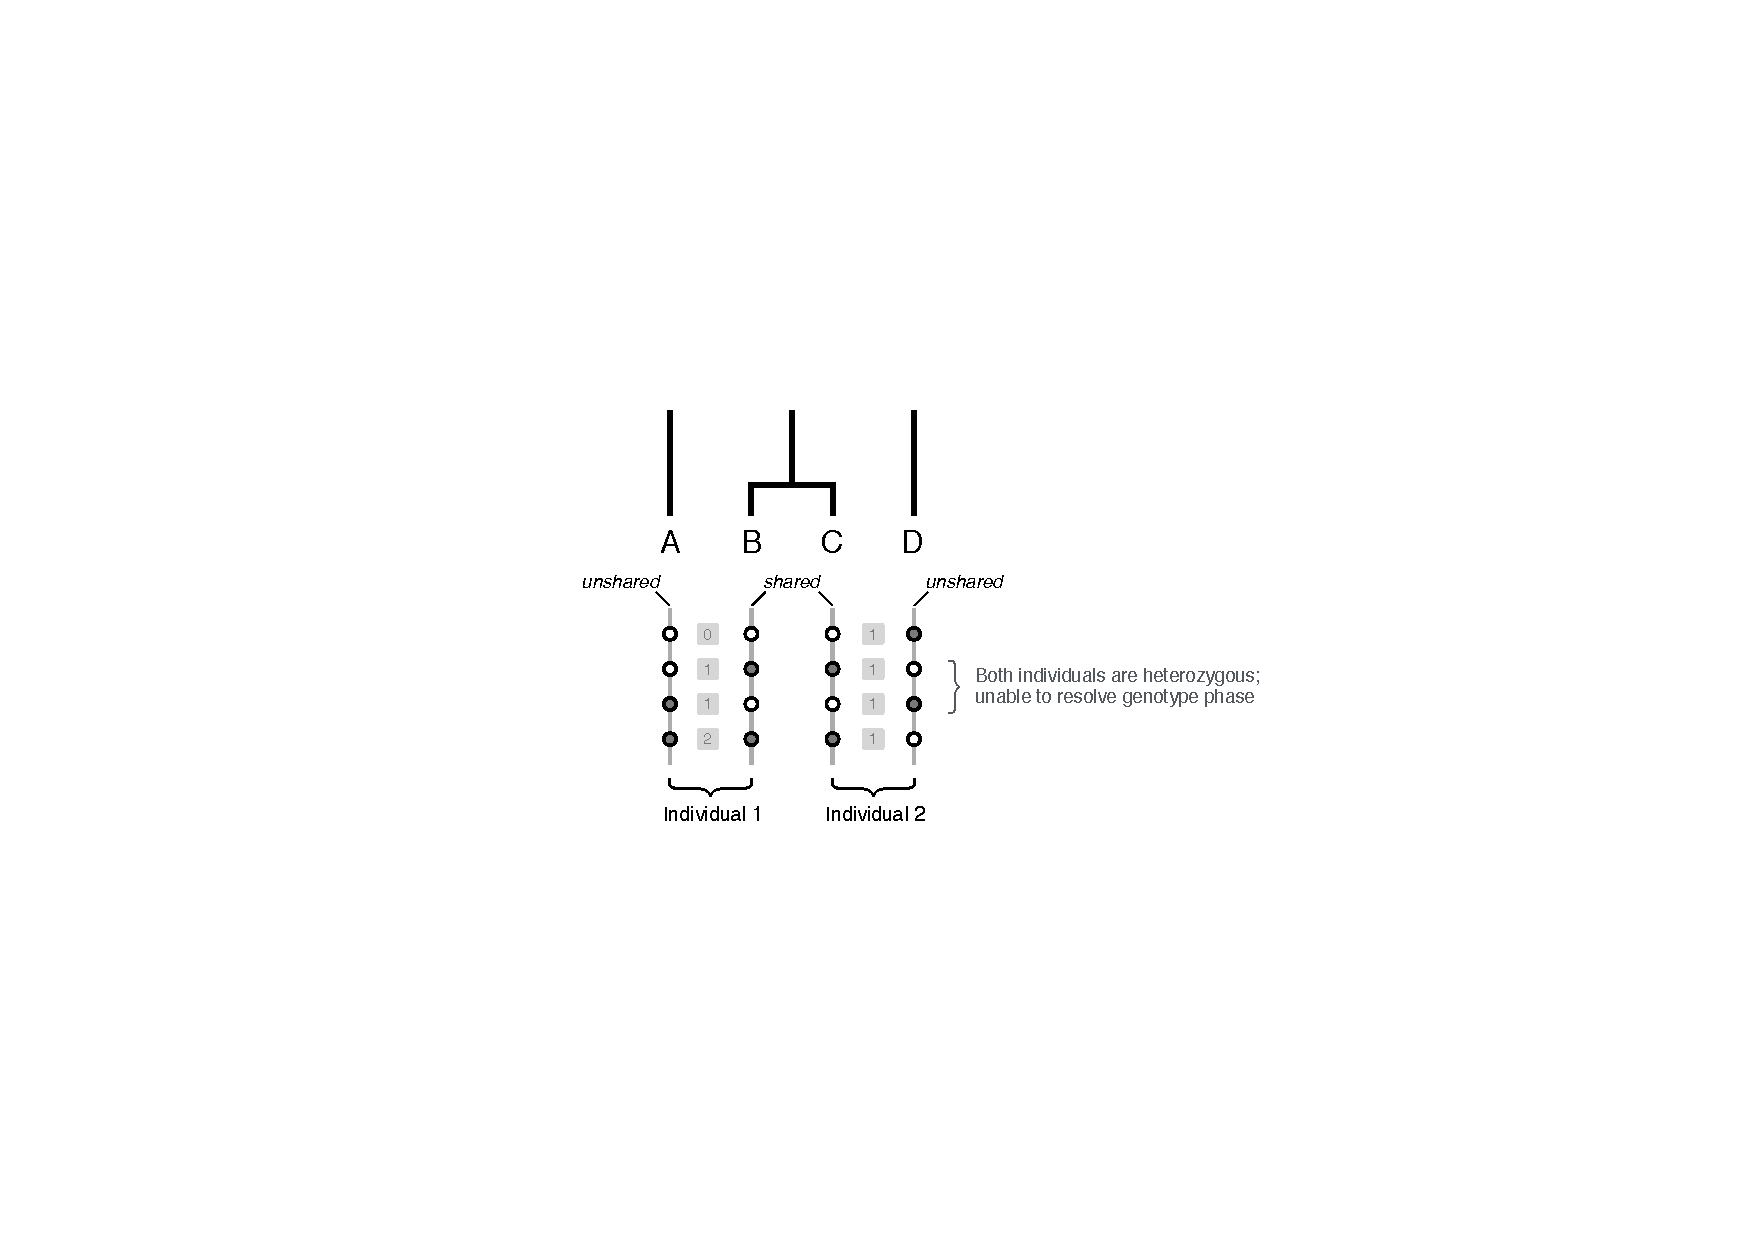
\includegraphics[width=0.75\textwidth]{./img/ch3/info_phase_pedigree}
\Caption{Genealogical constraints from haplotype sharing}
{The top graph indicates the genealogy of \n{4} haplotypes (A, B, C, and D) as seen in \n{2} individuals (1 and 2), which can be resolved partially if \n{2} haplotypes are shared by descent.
Below, the allelic states are shown at \n{4} positions along the sequence for each haplotype; ancestral and derived states are indicated by \emph{hollow} and \emph{solid} circles.
Only the genotypic state is seen in each individual as indicated between individual haplotypes; \ie homozygous for the ancestral allele (0), heterozygous (1), and homozygous for the derived allele (2).
The phase of a genotype can be resolved at sites with \n{1} homozygous genotype (phasing is redundant if both genotypes are homozygous).
Genotype phase cannot be determined if both individuals are heterozygous.}
{fig:info_phase_pedigree}
\end{figure}

% %
%
% A set of rules can be formulated which define the state of the shared allele if a certain genotype pair is observed in the \n{2} individuals considered.
% As before, the infinite sites model is assumed.
% If both genotypes are homozygous for the same allele, the deduction of the shared allele is trivial.
% If they are homozygous for different alleles, they cannot share an allele.
% Importantly, because this is seen at breakpoint sites detected using the \gls{dgt}, which mark the limits of the underlying IBD segment, breakpoints are excluded from this analysis; recall that the \gls{fgt} cannot be used with genotype data.
% A caveat of this analysis, however, is that haplotypes cannot be distinguished if both individuals are heterozygous, as it is not known whether the allele is shared or not.
% This conflict arises because an unshared haplotype may be more closely related to either the shared or the other unshared haplotype.
% Thus, haplotype inference is restricted to sites at which \emph{heterozygous-homozygous} genotype pairs are found.
% This is further illustrated in \cref{fig:info_phase_pedigree}.
%
% %
% % !TEX root = ../../main.tex


\begin{table}[!htb]
\Caption{Shared haplotype inference from genotype pairs}
{Given the \n{2} genotypes observed at a pair of individuals (A and B), there are \n{9} possible ordered combinations of alleles.
The corresponding haplotypes are shown for both individuals (unordered).
Note that genotype phase cannot be resolved for individuals that are both heterozygous; \ie the corresponding certainty score is equal to $\rfrac{1}{2}$.
If a pair is homozygous for different alleles, they do not share a haplotype.}
{tab:shared_hap_rules}
\centering
\begin{tabular}{ccccc}
\toprule
Genotype & Genotype &  Haplotypes & Haplotypes & Shared  \\
Individual $A$ & Individual $B$ &  Individual $A$ & Individual $B$ & haplotype  \\
\midrule
0  &  0  &  $(0,0)$  &  $(0,0)$  &  0  \\
0  &  1  &  $(0,0)$  &  $(0,1)$  &  0  \\
0  &  2  &  $(0,0)$  &  $(1,1)$  &  -- \\
1  &  0  &  $(0,1)$  &  $(0,0)$  &  0  \\
1  &  1  &  $(0,1)$  &  $(0,1)$  &  -- \\
1  &  2  &  $(0,1)$  &  $(1,1)$  &  1  \\
2  &  0  &  $(1,1)$  &  $(0,0)$  &  -- \\
2  &  1  &  $(1,1)$  &  $(0,1)$  &  1  \\
2  &  2  &  $(1,1)$  &  $(1,1)$  &  1  \\
\bottomrule
\end{tabular}
\end{table}

% %
%
% A complete definition of these rules is given in \cref{tab:shared_hap_rules}.
% The table gives the inferred allelic state of the shared haplotype for each of the possible combinations of \n{2} genotypes.
% Note that the alleles at \emph{heterozygous-heterozygous} sites are likely to be shared if \n{3} conditions are met; first, if the allele frequency at that site is lower than the frequency at the target position, second, if the allele only segregates within the subsample sharing the focal allele and, third, if the genealogy does not change along the sequence within an inferred interval.
% An allele that is lower in frequency is likely to be younger than the focal allele and, thus, to \Correct{be shared by some of the haplotypes within the sub-tree of the focal mutation}.
% However, this may only be the case under the infinite sites model, \eg because recurrent or back mutation may otherwise suggest a different genealogical order of descent.
%



%
\section{Evaluation}
%

The IBD detection method presented in this chapter was evaluated using simulated data.
This allowed assessment of the accuracy of detected breakpoint intervals in relation to the known genealogy of the simulated sample.
For comparison, an alternate IBD detection method was applied to the same data.
Lastly, the method presented was applied to data from the \glsentrylong{1kg}.



%
\subsection{Data generation}
\label{sec:msprime}
%

The coalescent simulator used to generate data was \texttt{msprime} (version~{0.4.0}), which simulates the exact coalescent with recombination, and where mutations are generated under the infinite sites model \citep{Kelleher:2016fn}.\footnote{Coalescent simulator \texttt{msprime}: \url{https://github.com/jeromekelleher/msprime} \accessed{2016}{11}{12}}
The software is a reimplementation of the classic \texttt{ms} algorithm by \citet{Hudson:2002vy}, but allows efficient simulation of extended chromosomal regions for very large sample sizes, where the entire history of the simulated sample can be stored and queried for further analysis.
Notably, \texttt{msprime} allows simulation under variable recombination rates, for example by using established recombination maps of the human genome.


%
\subsubsection{Demographic model}
\label{sec:sim_demo_model}
%

A demographic model was defined following \citet{Gutenkunst:2009gs}, who used intergenic data from \n{4} global populations to estimate parameters from diffusion approximations of expected allele frequency spectra.
Accordingly, here, data were simulated with an ancestral population size of ${\Ne = \num{7300}}$ (denoted by $N_A$ in the model) and under the assumption of a generation time of 25 years.
The mutation rate was set to a constant ${\mu = \num[round-precision=2]{2.35e-8}}$ per site per generation, which was estimated from the human-chimp divergence in \citet{Gutenkunst:2009gs}.
Note that recent studies have estimated the human mutation rate to be slightly lower; for example, \citet{Scally:2012fe} have estimated ${\mu \approx \num[round-precision=1]{1.2e-8}}$ from analyses of genome-wide \emph{de~novo} mutations using recent sequencing technologies, but which is in the same order as the mutation rate used here.

%
%!TEX root = ../../main.tex


\begin{figure}[!htb]
\centering
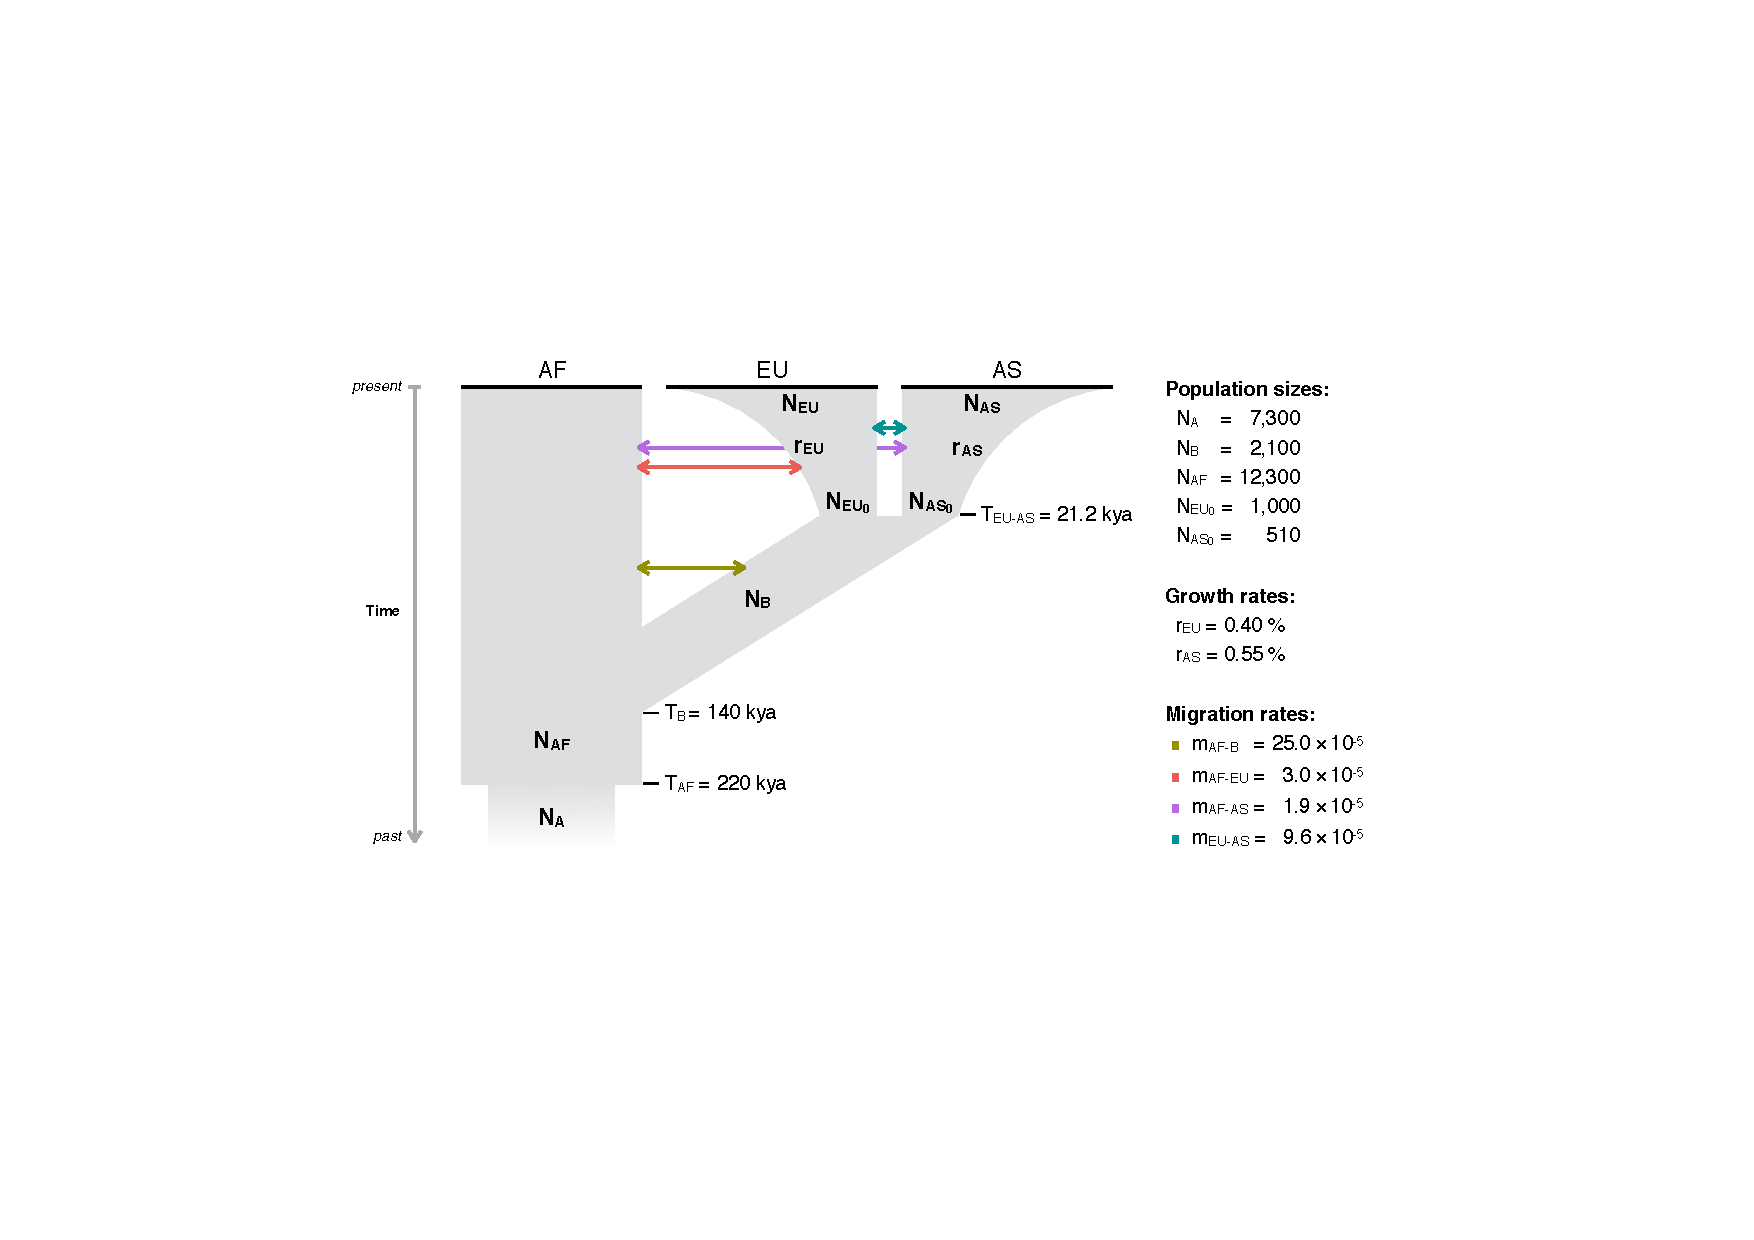
\includegraphics[width=0.95\textwidth]{./img/ch3/demo_model}
\Caption{Demographic model used in simulations}
{\N{3} populations were modelled, African (AF), European (EU), and Asian (AS), which derive from an ancestral population (A).
Both EU and AS experienced a bottleneck with subsequent exponential growth following the out-of-Africa expansion of a founder population (B) that split from the ancestral population.
Modified from \citet{Gutenkunst:2009gs}, Figure~2 (see \url{doi:10.1371/journal.pgen.1000695.g002}), with parameter values taken from Table~1 (see \url{doi:10.1371/journal.pgen.1000695.t001}).}
{fig:demo_model}
% \vspace{-5pt}
% \hrulefill%
\end{figure}

%

The demographic history as defined in the simulation model is illustrated in \cpref{fig:demo_model}; parameter values of the model are specified therein.
The model recapitulates the human expansion out of Africa, for which \n{3} populations were considered; African (AF), European (EU), and Asian (AS).
The African population was included with a constant population size, while EU and AS experienced exponential growth after divergence and split from an ancestral African population.
Population sizes of EU and AS were calculated as ${N = \rfrac{N_0}{\euler{-r t}}}$, where $N$ is the size at present, $N_0$ the initial size at EU-AS divergence, $r$ the growth rate, and $t$ the time since divergence (in years).


%
\subsubsection{Simulated dataset}
%

A sample of \n{5000} haplotypes was simulated, where the set of generated chromosomes represented a sample taken from the EU population.
To reproduce realistic distributions of recombination variability along the simulated sequence, the simulation was performed using recombination rates from human chromosome~20, as provided in Build~37 of the \gls{hapmap} Phase~\rom{2} \citep{Frazer:2007kha, InternationalHapMapConsortium:2010en}.\footnote{HapMap recombination map: \url{ftp://ftp.ncbi.nlm.nih.gov//hapmap/recombination/2011-01_phaseII_B37/genetic_map_HapMapII_GRCh37.tar.gz} \accessed{2016}{11}{12}}
The resulting dataset consisted of \dec{0.672847}~million segregating sites observed over a chromosomal length of \SI{62.949301}{\mega\basepair} (\SI{108.26675653}{\centi\morgan}).
The history of the simulated sample was stored separately to derive genealogical information in subsequent analyses.

The simulated chromosomes were used to generate \n{3} datasets.
In the first, haplotypes were randomly paired to construct a sample of \n{2500} diploid individuals.
From this, second, a corresponding genotype dataset was generated by forming genotypes (encoded as 0, 1, and 2) as the sum of alleles (encoded as 0 and 1) along the sequence in each individual.
This dataset was then used to generate a third dataset in which haplotypes were estimated from genotype data;
\ie resulting data consisted of phased haplotypes.
Phasing was conducted using \texttt{SHAPEIT} version~2 \citep{Delaneau:2008dk,Delaneau:2013hi}, using default parameters without a reference panel.\footnote{Phasing software \texttt{SHAPEIT}: \url{https://mathgen.stats.ox.ac.uk/genetics_software/shapeit/shapeit.html} \accessed{2016}{11}{12}}


%
\subsection{Accuracy analysis}
\label{sec:ibd_analysis}
%

The detection of IBD was evaluated in relation to the underlying true IBD structure of the sample, which was determined from the stored simulation records.
Given a target site and the \n{2} haplotypes sharing the focal allele, the genealogy was scanned along the sequence of variant sites observed in the sample, in both directions from the target position.
The \gls{mrca} of the pair was identified at each variant site and a breakpoint was defined as the first site at which a different \gls{mrca} was found.
This returned the smallest interval detectable from available data around the nearest recombination events that delimit an IBD segment.

Accuracy was measured in terms of the distance between a given breakpoint site and the focal position of the segment.
\N{2} measurements were considered; the squared Pearson correlation coefficient, $r^2$, which measures the strength of the linear relation between detected and true distance, and the \gls{rmsle};
\begin{equation}\label{eq:rmsle}
	\rmsle = \sqrt{ \frac{1}{n} \sum_{i=1}^n \Big[\log_{10}\Big(\frac{\hat{d}_i + 1}{d_i + 1}\Big)\Big]^2 }
\end{equation}
where $d_i$ and $\hat{d}_i$ are the distances of the true and detected breakpoints, respectively, and $n$ is the overall number of comparisons.
The \gls{rmsle} is similar to the root mean squared error (RMSE), which measures the variance and bias in the set of compared values, and is equal to the standard deviation when there is no bias.
As such, the \gls{rmsle} can be interpreted as a score metric for the magnitude of error.
Here, this is useful because larger departures from the actual values are penalised more than smaller ones.
A lower score value indicates a lower magnitude of error, where ${\rmsle = 0}$ indicates that true and inferred values are identical.
Also, note that the \gls{rmsle} is usually defined using the natural logarithm; here, $\log_{10}$ was used as a more intuitive representation of error magnitude.



The performance of the proposed IBD detection method was assessed for the described haplotype and genotype-based tests on the \n{3} datasets derived from coalescent simulations.
The following approaches were distinguished:
\begin{approach}\setlength\itemsep{0em}
\item\label{app:fgt_h} \gls{fgt} on haplotype data as simulated; \ie \emph{true} haplotypes,
\item\label{app:fgt_p} \gls{fgt} on \emph{phased} haplotypes, and
\item\label{app:dgt} \gls{dgt} on genotype data.
\end{approach}


%
\section{Results}
\label{sec:ibd_results}
%

IBD detection was carried out on a large set of target sites, for which all \fk{} variants found at ${k \in \lbrace 2, \ldots, 25 \rbrace}$ were selected, \ie alleles shared at frequency ${\leq 0.5\%}$.
This threshold was chosen arbitrarily, but such that the considered frequency range was expected to be sufficiently low to identify recent IBD given the size of the sample.
The set of target sites comprised \dec{0.317020}~million \glspl{snp} that were heterozygous in the individuals sharing a focal allele.
This resulted in \dec{11.597968}~million pairwise analyses and an equal number of IBD segments detected using the \gls{fgt} on the true and phased haplotypes in \cref{app:fgt_h,,app:fgt_p}, respectively, and the \gls{dgt} on genotype data in \cref{app:dgt}.

Because the same IBD segment may be inferred from multiple target sites, the analysis was reduced to the set of uniquely detected breakpoint intervals per pair of individuals in each approach.
Duplicate segments were removed after the corresponding target variants were sorted by allele frequency, with lower frequencies at the top and removing duplicate segments below.
Detected segments were thereby tagged by the presumably youngest shared alleles within the intervals.
The number of uniquely identified segments differed slightly in \cref{app:fgt_h,,app:fgt_p,,app:dgt};
\dec{2.983342}~million (\SI{25.72297}{\percent}),
\dec{3.091288}~million (\SI{26.65370}{\percent}), and
\dec{2.978238}~million (\SI{25.67896}{\percent}), respectively.
For the corresponding true IBD segments, the number of unique segments was \dec{3.001053}~million (\SI{25.87568}{\percent}).
These data were further reduced to the intersection of retained target sites across approaches, so as to enable direct comparisons on the same set of targets, which resulted in \dec{2.978220}~million (\SI{25.67881}{\percent}) unique intervals.
The results obtained from these data are summarised in \cpref{tab:stat_breakpoints}.

%
% !TEX root = ../../main.tex


\begin{table}[!htb]
\Caption{Accuracy of detected breakpoints per $\textbf{f}_{k}$~category}
{The accuracy of detected IBD breakpoints was measured using the squared Pearson correlation coefficient, $r^2$, and the \gls{rmsle} in relation to the true IBD segments determined from simulation records; measured in terms of the distance between breakpoint site and the corresponding focal position per segment.
The analysis included of \n{317020} target sites around which IBD was detected in \cref{app:fgt_h,,app:fgt_p,,app:dgt}.
In each, accuracy was computed after data were reduced to identical sets of unique IBD segments (${n=\num{2978220}}$).
The table specifies the allele frequency~(\%) corresponding to each \fk{}~category, as well as the number of target sites identified.}
{tab:stat_breakpoints}
\centering
\begin{threeparttable}
\begin{tabular}{
cc
S[table-format=6.1]
*3{S[table-format=1.3]}
c
*3{S[table-format=1.3]}}
\toprule
\fk{} & Freq.~{\%} & \multicolumn{1}{c}{Targets} &
\multicolumn{3}{c}{$r^2$} & &
\multicolumn{3}{c}{$\rmsle$} \\
\cmidrule(lr){4-6}
\cmidrule(lr){8-10}
 & & &
 \multicolumn{1}{c}{\textsc{fgt}$^{\ast}$} &
 \multicolumn{1}{c}{\textsc{fgt}$^{\ast\ast}$} &
 \multicolumn{1}{c}{\textsc{dgt}$^{\dagger}$} & &
 \multicolumn{1}{c}{\textsc{fgt}$^{\ast}$} &
 \multicolumn{1}{c}{\textsc{fgt}$^{\ast\ast}$} &
 \multicolumn{1}{c}{\textsc{dgt}$^{\dagger}$} \\
\midrule
2  & 0.04 & 76515  &  \bfseries 0.99764 & 0.89458 & 0.99520  & &  \bfseries 0.21948 & 0.59833 & 0.31710 \\
3  & 0.06 & 46138  &  \bfseries 0.98869 & 0.95705 & 0.97784  & &  \bfseries 0.24316 & 0.51595 & 0.35887 \\
4  & 0.08 & 31658  &  \bfseries 0.96294 & 0.95872 & 0.94097  & &  \bfseries 0.25555 & 0.46282 & 0.37881 \\
5  & 0.10 & 23581  &  \bfseries 0.97480 & 0.96275 & 0.92906  & &  \bfseries 0.27554 & 0.42873 & 0.40830 \\
6  & 0.12 & 19241  &  \bfseries 0.95448 & 0.93766 & 0.90396  & &  \bfseries 0.28086 & 0.40886 & 0.42082 \\
7  & 0.14 & 15869  &  \bfseries 0.95501 & 0.94390 & 0.89159  & &  \bfseries 0.29827 & 0.40264 & 0.44651 \\
8  & 0.16 & 13175  &  0.89794 & \bfseries 0.91758 & 0.81310  & &  \bfseries 0.31984 & 0.39805 & 0.46935 \\
9  & 0.18 & 10966  &  \bfseries 0.93158 & 0.92740 & 0.82685  & &  \bfseries 0.31402 & 0.37511 & 0.46718 \\
10 & 0.20 & 11142  &  0.87942 & \bfseries 0.88681 & 0.77257  & &  \bfseries 0.33200 & 0.38713 & 0.49355 \\
11 & 0.22 &  9392  &  \bfseries 0.89481 & 0.89213 & 0.75844  & &  \bfseries 0.34414 & 0.40133 & 0.51339 \\
12 & 0.24 &  7751  &  0.83526 & \bfseries 0.84776 & 0.73282  & &  \bfseries 0.35792 & 0.39763 & 0.52569 \\
13 & 0.26 &  6933  &  \bfseries 0.84208 & 0.83534 & 0.72078  & &  \bfseries 0.36065 & 0.40463 & 0.53176 \\
14 & 0.28 &  5767  &  \bfseries 0.81623 & 0.81622 & 0.67937  & &  \bfseries 0.36694 & 0.39075 & 0.54006 \\
15 & 0.30 &  5062  &  \bfseries 0.87140 & 0.86023 & 0.71246  & &  \bfseries 0.38095 & 0.40601 & 0.55560 \\
16 & 0.32 &  4711  &  \bfseries 0.83929 & 0.82998 & 0.70121  & &  \bfseries 0.37271 & 0.39465 & 0.54617 \\
17 & 0.34 &  4210  &  0.82865 & \bfseries 0.83173 & 0.68057  & &  \bfseries 0.38680 & 0.41049 & 0.56620 \\
18 & 0.36 &  3913  &  0.81267 & \bfseries 0.83171 & 0.67040  & &  \bfseries 0.37969 & 0.39699 & 0.56071 \\
19 & 0.38 &  3684  &  \bfseries 0.80141 & 0.79804 & 0.64162  & &  \bfseries 0.38074 & 0.40128 & 0.56564 \\
20 & 0.40 &  3214  &  0.83058 & \bfseries 0.83677 & 0.68478  & &  \bfseries 0.40090 & 0.41599 & 0.58737 \\
21 & 0.42 &  3333  &  0.77276 & \bfseries 0.77758 & 0.60320  & &  \bfseries 0.39881 & 0.41259 & 0.58359 \\
22 & 0.44 &  2863  &  0.75260 & \bfseries 0.79505 & 0.57059  & &  \bfseries 0.39876 & 0.40632 & 0.58646 \\
23 & 0.46 &  2595  &  0.73156 & \bfseries 0.74493 & 0.59629  & &  \bfseries 0.41417 & 0.42509 & 0.59901 \\
24 & 0.48 &  2653  &  \bfseries 0.78359 & 0.77969 & 0.58121  & &  \bfseries 0.39649 & 0.40641 & 0.58343 \\
25 & 0.50 &  2654  &  0.70052 & \bfseries 0.72997 & 0.56030  & &  \bfseries 0.39960 & 0.40764 & 0.58521 \\
\bottomrule
\end{tabular}
\begin{tablenotes}\footnotesize
	\item[$\ast$] ~ \cref{app:fgt_h}, using the \gls{fgt} with true haplotypes
	\item[$\ast\ast$] ~ \cref{app:fgt_p}, using the \gls{fgt} with phased haplotypes
	\item[$\dagger$] ~ \cref{app:dgt}, using the \gls{dgt} with genotype data
\end{tablenotes}
\end{threeparttable}
\end{table}

% 21803
% 36501
% 49533
% 59157
% 69271
% 89298
% 86317
% 98192
% 106765
% 118180
% 121107
% 123542
% 132232
% 139403
% 146324
% 150165
% 147554
% 149660
% 162293
% 176537
% 187870
% 195883
% 162501
% 94297

% 18795
% 34042
% 47338
% 59683
% 69487
% 81376
% 91580
% 98374
% 105827
% 116829
% 123145
% 127134
% 130059
% 145055
% 147945
% 151803
% 157849
% 160246
% 164855
% 183665
% 177742
% 181959
% 195948
% 207484

%

The proportion of breakpoints that were overestimated (in relation to the corresponding true IBD breakpoints) was noticeably high overall; using the \gls{fgt}, \SI{97.3903}{\percent} and \SI{95.66553}{\percent} were overestimated in \cref{app:fgt_h,,app:fgt_p}, respectively.
However, overestimation was highest when the \gls{dgt} was used (\SI{98.36191}{\percent}) in \cref{app:dgt}.
Conversely, the proportion of underestimated breakpoints was lowest in \ref{app:dgt}, \SI{1.543153}{\percent}, and highest when haplotypes were phased in \ref{app:fgt_p}, \SI{4.146739}{\percent}; in \ref{app:fgt_h}, \SI{2.41782}{\percent} of breakpoints were underestimated.
The proportion of detected breakpoints that coincided with the corresponding true breakpoints was \SI{0.19180}{\percent}, \SI{0.187729}{\percent}, and \SI{0.094939}{\percent} in \ref{app:fgt_h}, \ref{app:fgt_p}, and \ref{app:dgt}, respectively.

% Accuracy was measured in terms of the distance between breakpoint site and the corresponding focal position per detected and true IBD segments.
The highest overall accuracy was found for the \gls{fgt} on true haplotypes, followed by the analysis on phased haplotypes, which had ${r^2 = \dec{0.9262482}}$ and ${r^2 = \dec{0.8922048}}$ in \cref{app:fgt_h,,app:fgt_p}, respectively.
The accuracy achieved by the \gls{dgt} was lower, but still considerably high with ${r^2 = \dec{0.8474036}}$ in \cref{app:dgt}.
This was also reflected in the measued magnitude of error (\gls{rmsle}), which was \dec{0.39983}, \dec{0.43407}, and \dec{0.56940} in \ref{app:fgt_h}, \ref{app:fgt_p}, and \ref{app:dgt}, respectively.
The measurement of accuracy was further broken down by the allele frequency of target variants (\fk{}~category); results are shown in \cpref{tab:stat_breakpoints}.
Accuracy decreased towards higher allele frequency in each approach.
For example, for \fk{2}~variants, $r^2$ was \dec{0.998}, \dec{0.985}, and \dec{0.995} in \ref{app:fgt_h}, \ref{app:fgt_p}, and \ref{app:dgt}, respectively,
which was reduced for \fk{25}~variants where ${r^2 = \dec{0.701}}$ in~\ref{app:fgt_h} and ${r^2 = \dec{0.730}}$ in~\ref{app:fgt_p}, but where \ref{app:dgt} was seen to decrease more rapidly by comparison (${r^2 = \dec{0.560}}$).
Notably, when haplotype data were phased in \ref{app:fgt_p}, accuracy was highest at \fk{5}~variants (${r^2 = \dec{0.963}}$), indicating that accuracy was decreased at lower frequencies.
Similarly, \gls{rmsle} scores reflected the same general pattern, but where the magnitude of error in \ref{app:fgt_p} was at a maximum at \fk{2}~variants.

%
% !TEX root = ../../main.tex


\begin{figure}[!htbp]
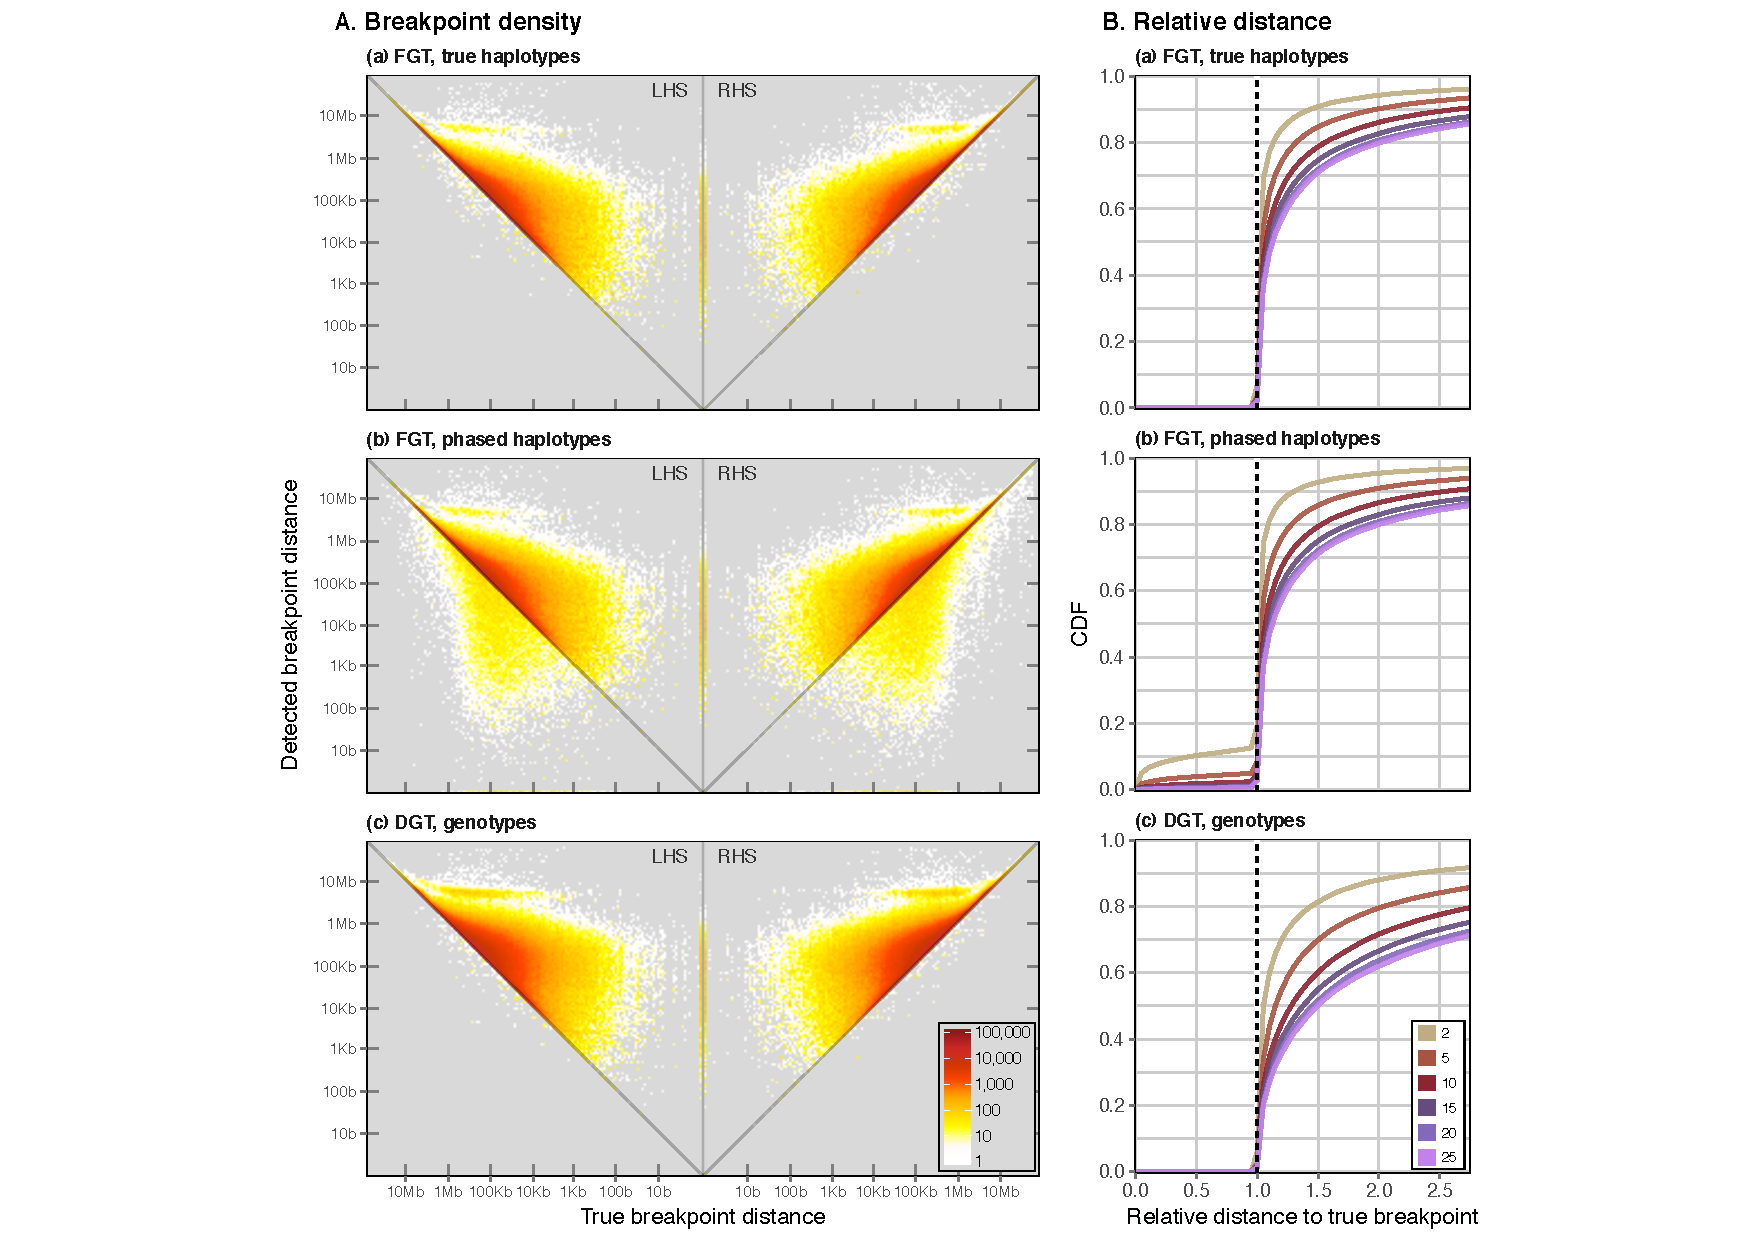
\includegraphics[width=\textwidth]{./img/ch3/naive_break_tru.pdf}
\Caption{Accuracy of breakpoint detection in simulated data}
{Breakpoints detected in \fk{} pairs at ${k \in \lbrace 2, \ldots, 25 \rbrace}$ are compared to true IBD breakpoint sites, after removing boundary cases in either the detected or true dataset.
Segments were inferred using the \gls{fgt} on true haplotypes \textbf{(a)} and phased haplotypes \textbf{(b)}, as well as the \gls{dgt} on genotype data \textbf{(c)}.
Panel~\textbf{(A)} illustrates the relationship between each detected breakpoint and the corresponding true breakpoint, measured as the physical distance to the focal site.
Along each axis, distances were pooled into \n{200} bins (on log scale)
and cells in the resulting $200^2$ grid were colour-coded for the number of  intersecting true and detected breakpoints, where grey indicates zero.
Segment breakpoints to the left (\emph{LHS}) and right-and side (\emph{RHS}) of the focal position are shown separately.
Panel~\textbf{(B)} shows the \gls{cdf} of detected breakpoints in relative distance to the focal and true breakpoint sites.
The physical distance between detected breakpoint and focal position was divided by the distance between true breakpoint and focal position, such that values $<1$ indicate underestimation and $>1$ overestimation relative to the true distance (\emph{dashed line}).}
{fig:naive_break_tru}
% \vspace{-5pt}
% \hrulefill
\end{figure}

%

A more intuitive representation of results is provided in \cpref{fig:naive_break_tru}, which compares true and detected breakpoint distances in \n{2} ways.
First, in \cref{fig:naive_break_tru}{A}, breakpoint densities are shown in separate scatterplots for breakpoints detected on the left and right-hand side of focal positions.
For example, a clear difference in the proportion of underestimated breakpoints can be seen between \cref{app:fgt_h,,app:fgt_p}, \ie where the \gls{fgt} was used on true and phased haplotypes, respectively.
In \cref{app:dgt}, where the \gls{dgt} was used on genotype data, breakpoint densities indicate a higher proportion of overestimated distances compared to \ref{app:fgt_h} or \ref{app:fgt_p}.
Second, in \cref{fig:naive_break_tru}{B}, the relative distance was calculated as ${x=\rfrac{\hat{d}_i}{d_i}}$, where $\hat{d}$ and $d$ denote detected and true distances, respectively.
By doing so, detected breakpoint distances were ``mapped'' relative to the corresponding true distances, such that ${0<x<1}$ indicates underestimation and ${x>1}$ indicates overestimation.
The \gls{cdf} of the relative distance is shown separately per \fk{}~category.
For example, it can be seen that a larger proportion of \fk{2}~variants (\SI{15.21486}{\percent}) contributed to the overall underestimation found in \cref{app:fgt_p}, \eg compared to \fk{5} (\SI{5.543963}{\percent}) and \fk{25}~variants (\SI{0.755359}{\percent}).


%
% !TEX root = ../../main.tex


\begin{figure}[!htb]
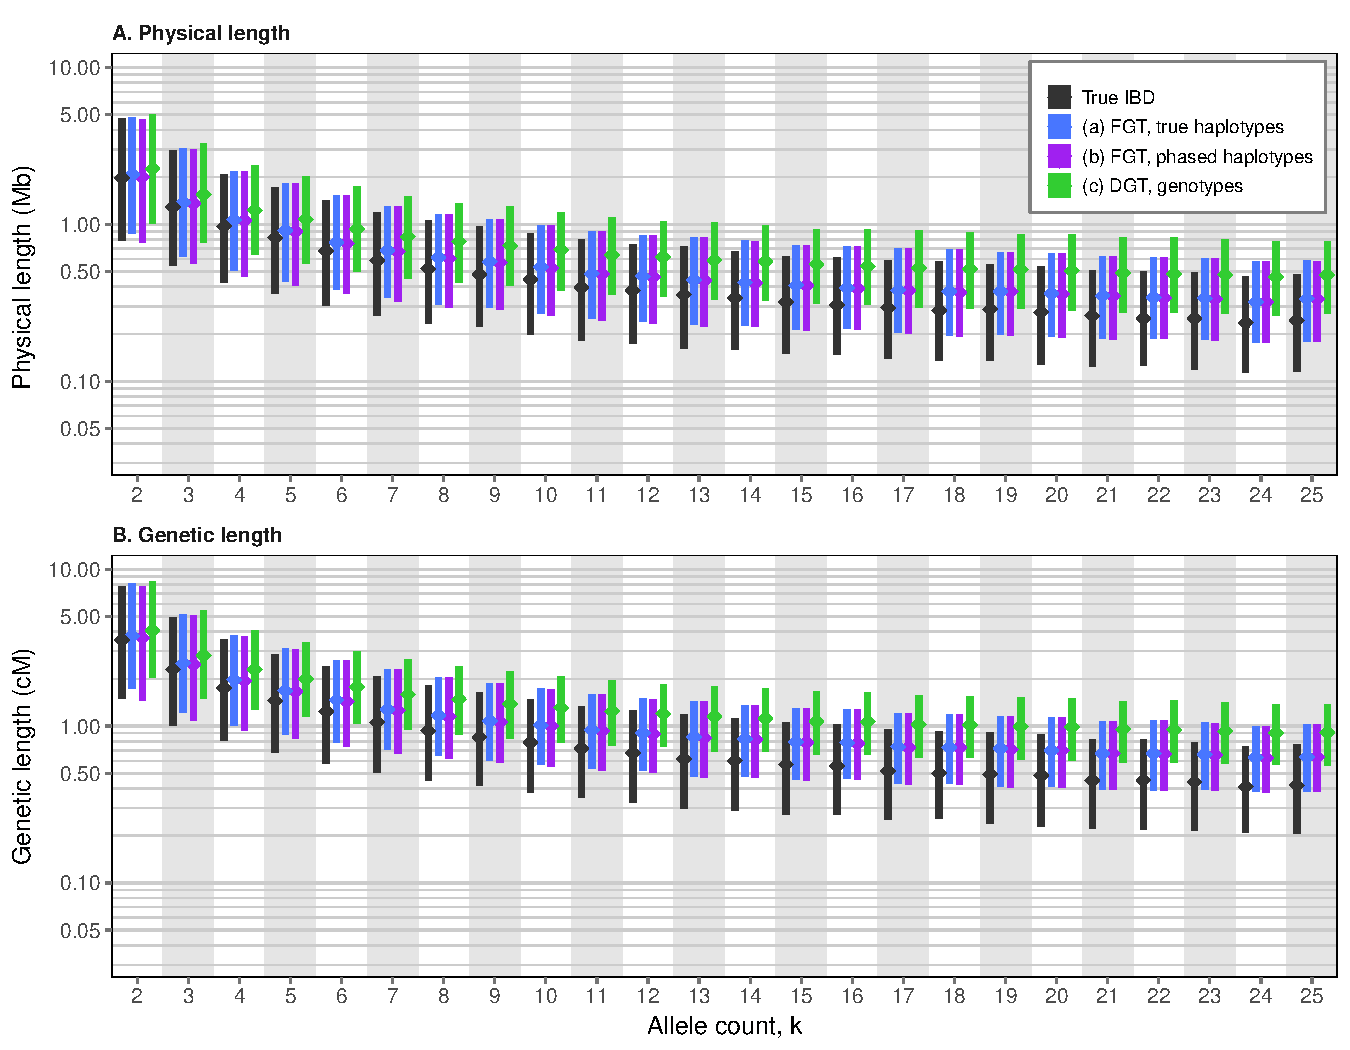
\includegraphics[width=\textwidth]{./img/ch3/naive_length_tru}
\Caption{IBD segment lengths inferred in simulated data}
{The distribution of median physical and genetic length of detected IBD segments is shown by allele frequency of the focal variant (\fk{[2,25]}).
IBD detection was performed using the \gls{fgt} on true and phased haplotypes, as well as the \gls{dgt} on genotype data; \cref{app:fgt_h,,app:fgt_p,,app:dgt}, respectively.
The true IBD length is shown for comparison.
Bottom and top of each bar indicate \nth{1} and \nth{3} quartiles, respectively, between which the median (\nth{2} quartile) is marked (\emph{diamonds}).}
{fig:naive_length_tru}
\end{figure}

%

The distribution of physical and genetic IBD length is shown in \cpref{fig:naive_length_tru}.
These results were obtained after boundary cases were removed in each approach (\ie discarding segments where the end of a chromosome was reached without detecting a breakpoint), so as to ensure that observed IBD length was delimited by recombination on both sides of a segment; \SI{1.448516}{\percent}, \SI{1.400165}{\percent}, and \SI{1.636716}{\percent}
were removed in \ref{app:fgt_h}, \ref{app:fgt_p}, and \ref{app:dgt}, respectively, and \SI{1.339693}{\percent} in the set of true IBD segments.
Data were then intersected again to retain the same set of target sites in each approach; as a result, \dec{2.929475}~million unique segments were retained (\SI{98.363284}{\percent}).

Median physical length (and median genetic length) over the set of retained segments was computed for each approach.
A small difference was seen for the \gls{fgt}, where median length was
\SI{0.4174283}{\mega\basepair} (\SI{0.8000373}{\centi\morgan})
on true haplotypes in \cref{app:fgt_h}, and
\SI{0.4126863}{\mega\basepair} (\SI{0.7905954}{\centi\morgan})
on phased haplotypes in \cref{app:fgt_p}.
For the \gls{dgt} on genotype data, median length was longer by comparison, \SI{0.5703613}{\mega\basepair} (\SI{1.0938442}{\centi\morgan}).
The median of true IBD length was \SI{0.3281641}{\mega\basepair} (\SI{1.5733807}{\centi\morgan}), which was shorter than detected in each approach.
But as seen in \cref{fig:naive_length_tru}, the distribution of IBD lengths in \ref{app:fgt_h}, \ref{app:fgt_p}, and \ref{app:dgt} closely followed the true lengths along the allele frequency range.
However, the gap between true and detected lengths increased towards higher allele frequencies.
For example, for \fk{2}~variants, median length of true IBD segments was
\SI{1.9775512}{\mega\basepair} (\SI{3.5510944}{\centi\morgan}),
which is only marginally shorter compared to
\SI{2.0786201}{\mega\basepair} (\SI{3.7725436}{\centi\morgan}),
\SI{2.0053149}{\mega\basepair} (\SI{3.6522954}{\centi\morgan}), and
\SI{2.2558099}{\mega\basepair} (\SI{4.0847501}{\centi\morgan})
in \ref{app:fgt_h}, \ref{app:fgt_p}, and \ref{app:dgt}, respectively.
For \fk{25}~variants the difference was more pronounced; \ie
median length of true IBD segments was
\SI{0.2433351}{\mega\basepair} (\SI{0.4194589}{\centi\morgan}),
compared to
\SI{0.3358179}{\mega\basepair} (\SI{0.6359137}{\centi\morgan}),
\SI{0.3345750}{\mega\basepair} (\SI{0.6338472}{\centi\morgan}), and
\SI{0.4750292}{\mega\basepair} (\SI{0.9073333}{\centi\morgan})
in \ref{app:fgt_h}, \ref{app:fgt_p}, and \ref{app:dgt}, respectively.


In summary, the \gls{fgt} on true haplotype data in \cref{app:fgt_h} overall achieved the highest levels of accuracy while maintaining low error.
This was particularly seen in comparison to \cref{app:fgt_p}, which differed only in the additionally included phasing step.
Since genomic datasets were typically composed of phased haplotypes, \cref{app:fgt_p} can be seen as being the realistic approach.
However, the higher error rate at lower frequency variants may pose a problem for analysis for rare variants.
As an alternative, the \gls{dgt} on genotype data, \cref{app:dgt}, can be used to detect IBD with high accuracy and comparatively low error rates.
However, the larger proportion of overestimated IBD breakpoints may result in additional error, \eg if it is assumed that the genealogy is consistent along the sequence of inferred IBD segments.




%
\subsubsection{IBD detection using the \emph{Refined\,IBD} algorithm}
\label{sec:ibd_beagle_tru}
%

Simulated data were additionally analysed using the \texttt{Refined\,IBD} algorithm implemented in \texttt{Beagle} version~4.1 \citep{Browning:2013eh}.\footnote{Beagle 4.1: \url{https://faculty.washington.edu/browning/beagle/beagle.html} \accessed{2016}{11}{22}}
The method is based on the non-probabilistic \texttt{GERMLINE} algorithm \citep{Gusev:2009hd}, which identifies putative IBD segments from short exact matches between haplotype pairs; candidate segments are found by extending identified regions to longer inexact matches.
In \texttt{Refined\,IBD}, an additional probabilistic approach is included to assess candidate segments conditional on the \gls{lr} of the data, calculated under IBD and non-IBD models.
A \gls{lod} score is calculated as ${\log_{10}(\text{LR})}$, and segments are reported as IBD if the \gls{lod} score is above a specified threshold.
This approach has been found to achieve greater accuracy than \texttt{GERMLINE} alone or \texttt{fastIBD}, which is a non-probabilistic method that detects IBD based on haplotype frequency \citep{Browning:2011do,Browning:2013eh}.

The analysis was performed using default parameters in \texttt{Refined\,IBD} (retaining candidate segments at ${\mbox{LOD}>3.0}$) and after conversion of simulated data into \gls{vcf}\footnote{Variant Call Format: \url{http://vcftools.sourceforge.net/VCF-poster.pdf} \accessed{2016}{11}{22}}.
Note that haplotype data are required; therefore only the \gls{fgt} was evaluated using true and phased haplotype data in \cref{app:fgt_h,,app:fgt_p}, respectively.
The analysis returned \dec{13.688781}~million IBD segments in \ref{app:fgt_h}, of which \SI{0.248108}{\percent} were duplicated, and \dec{13.647038}~million in \ref{app:fgt_p}, of which \SI{0.248933}{\percent} were duplicated.
The median length of all detected segments was \SI{0.190912}{\mega\basepair} and \SI{0.191496}{\mega\basepair} in \ref{app:fgt_h} and \ref{app:fgt_p}, respectively (after removal of duplicates).

The accuracy of detected IBD segments was measured in relation to the true IBD intervals, which were already determined for the set of previously analysed target sites; \ie all \fk{[2,25]} variants found in the data (allele frequency $\leq 0.5\%$).
Note that the detection approach employed by \texttt{Refined\,IBD} reports all segments inferred for a given pair of haplotypes, such that detected and true intervals cannot be matched by direct reference to a particular target site.
Hence, for a given pair of haplotypes, true and detected segments were matched if the focal allele associated with a true segment fell within the interval of the detected segment, which was discarded if none of the pairwise shared target alleles were found within the detected interval.
This matching process resulted in a set of \dec{2.166492}~million unique segments in the analysis conduced on true haplotypes, \cref{app:fgt_h}.
% This number is low when seen in relation to the full set of unique segments detected (\SI{0.1586614}{\percent}), but reasonably large in relation to the set of true unique segments available (\SI{72.19106}{\percent}).
For the phased dataset, \cref{app:fgt_p}, \dec{0.528477}~million unique segments were matched.
% , which corresponded to a lower proportion of retained segments in relation to both the full set (\SI{3.917097}{\percent}) and the set of true segments (\SI{17.76833}{\percent}).
The lower number of segments retained in \cref{app:fgt_p} is likely to be the consequence of mismatched haplotypes in original and phased data.

After the removal of segments at which haplotype pairs did not share any of the alleles in \fk{[2,25]}, median lengths were longer in comparison to the original datasets; \SI{0.255496}{\mega\basepair} and \SI{0.256070}{\mega\basepair} in \ref{app:fgt_h} and \ref{app:fgt_p}, respectively.
This can be seen as the result of both the removal of falsely identified segments, as well as segments that were older and thereby expected to be shorter.

%
% !TEX root = ../../main.tex


\begin{figure}[tb]
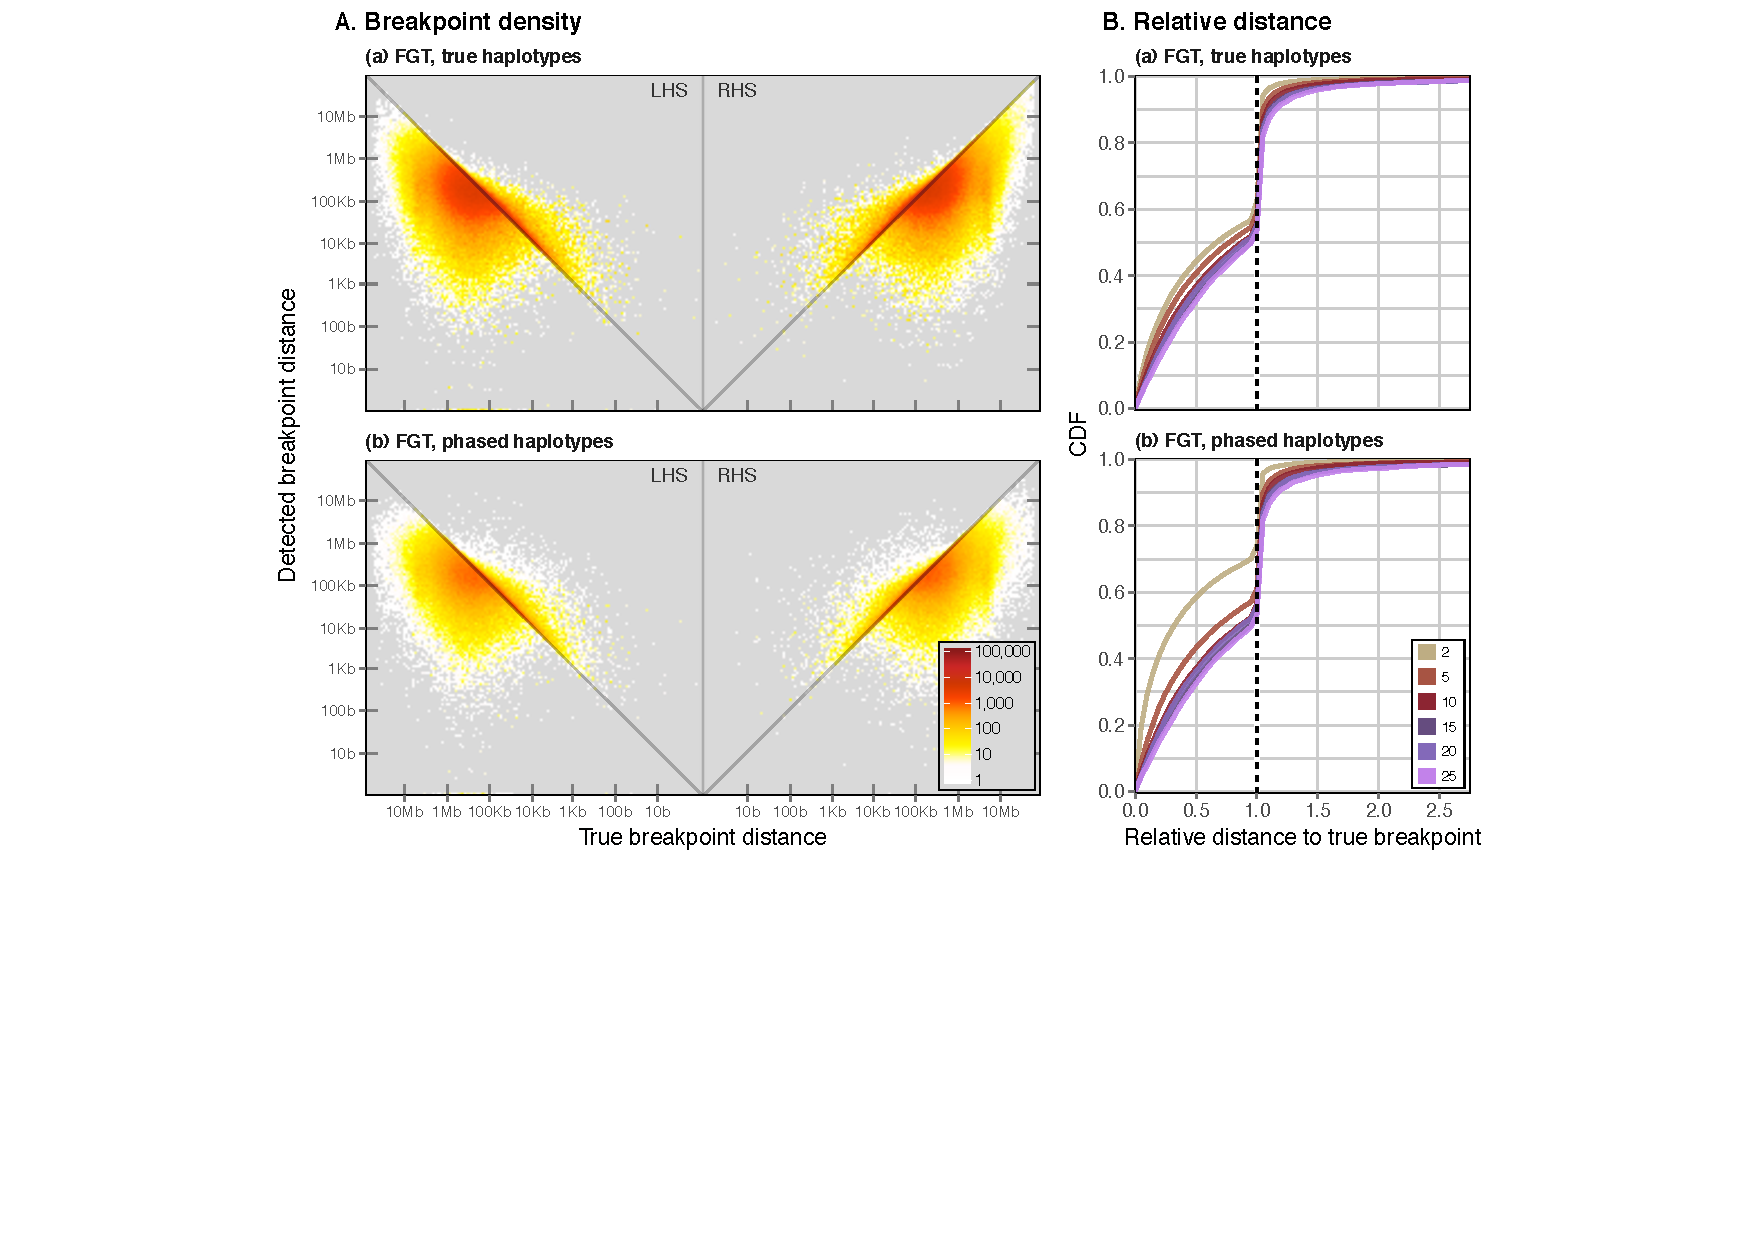
\includegraphics[width=\textwidth]{./img/ch3/beagle_break_tru}
\Caption{Accuracy of breakpoint detection in simulated data using Refined IBD in Beagle~4.1}
{Results are shown for uniquely detected shared haplotype segments inferred using the Refined IBD method; after removing boundary cases in either the detected or true segments, and after the detected segments were matched to the set of true segments.
Segments were inferred on true (simulated) haplotype data \textbf{(a)} and phased haplotypes \textbf{(b)}.
Panel~\textbf{(A)} provides a heatmap representation of a scatter plot, comparing physical distances between focal site and true breakpoint (x-axis) and detected breakpoint (y-axis).
Segment breakpoints to the left (\emph{LHS}) and right-and side (\emph{RHS}) of the focal position are shown separately.
Panel~\textbf{(B)} shows the \gls{cdf} of detected breakpoints in relative distance to the focal and true breakpoint sites.}
{fig:beagle_break_tru}
% \vspace{-5pt}
% \hrulefill%
\end{figure}

%

The majority of retained breakpoints was underestimated in both \cref{app:fgt_h,,app:fgt_p}; \SI{55.35559}{\percent} and \SI{56.60644}{\percent}, respectively.
In \cref{app:fgt_h}, \SI{44.38505}{\percent} were overestimated and \SI{0.2593594}{\percent} coincided with true breakpoint positions.
This was similar in \cref{app:fgt_p}, where \SI{43.15511}{\percent} were overestimated and \SI{0.2384493}{\percent} coincided.
Accuracy was measured in terms of the physical distance between breakpoint position and the corresponding focal site.
Because the latter was not specified in the results obtained from \texttt{Refined\,IBD}, the same focal position as associated with the matched true IBD segment was assumed.
Data were not reduced to the intersection of segments retained across datasets, due to the low number of consistent matches.
These results are illustrated in \cpref{fig:beagle_break_tru}.

The distance distribution of true and detected breakpoints (\cref{fig:beagle_break_tru}{A}) suggests that detected breakpoints were closely distributed around the corresponding true breakpoints.
However, overall accuracy was low in both \ref{app:fgt_h} and \ref{app:fgt_p}, reaching ${r^2 = \dec{0.2868218}}$ and ${r^2 = \dec{0.1707155}}$, respectively.
The magnitude of error, \gls{rmsle}, was lower in \ref{app:fgt_h} compared to \ref{app:fgt_p}; \dec{0.5954253} and \dec{0.6158843}, respectively.
When true haplotypes were analysed, \cref{app:fgt_h}, accuracy decreased steadily towards higher allele frequencies.
For example, accuracy was highest for \fk{2}~variants (${r^2 = \dec{0.34591189}}$) but lowest for \fk{25}~variants (${r^2 = \dec{0.07445725}}$).
However, the magnitude of error was highest for \fk{2}~variants (${\rmsle = \dec{0.7498976}}$) and lowest for \fk{25}~variants (${\rmsle = \dec{0.5433645}}$).
When haplotypes were phased, \cref{app:fgt_p}, error was further increased at \fk{2}~variants (${\rmsle = \dec{0.999}}$) in comparison to \fk{25}~variants (${\rmsle = \dec{0.5456303}}$).
The higher error at lower allele frequencies was also reflected in $r^2$~values; \eg accuracy was low at \fk{2} (${r^2 = \dec{0.08720971}}$), higher at \fk{5} (${r^2 = \dec{0.13222751}}$), but lowest at \fk{25} (${r^2 = \dec{0.04827430}}$).
The difference between true and phased datasets is further highlighted in  \cref{fig:beagle_break_tru}{B}, where a higher proportion of \fk{2}~variants is seen to be underestimated in \ref{app:fgt_p}.

%
% !TEX root = ../../main.tex


\begin{figure}[!htb]
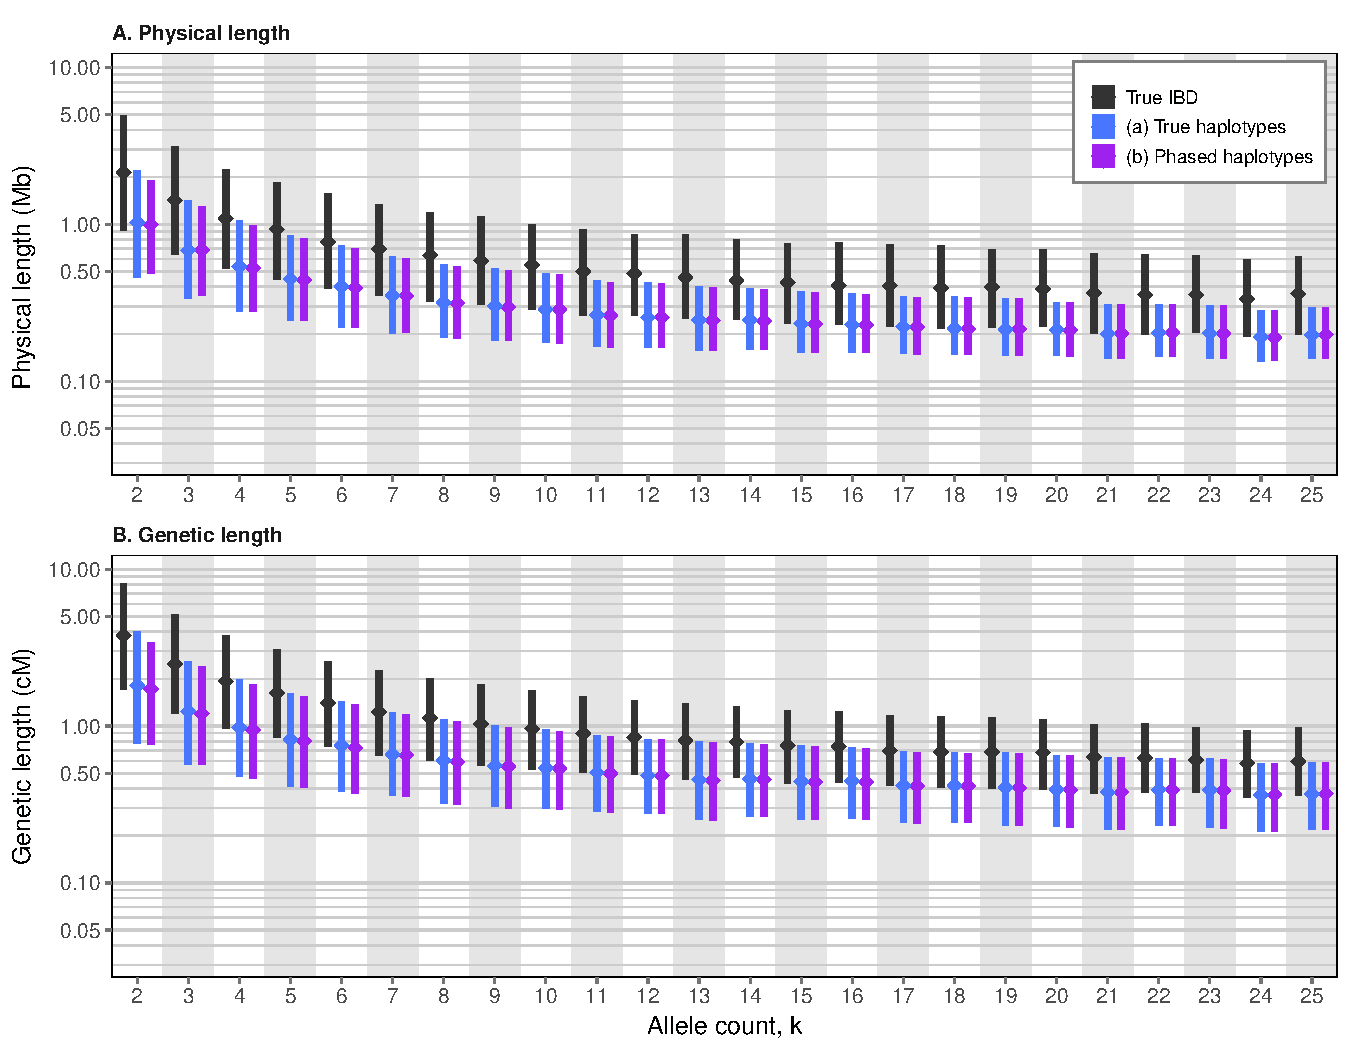
\includegraphics[width=\textwidth]{./img/ch3/beagle_length_tru_new}
\Caption{IBD segment lengths inferred using \emph{Refined\,IBD} in Beagle~4.1}
{The distribution of median physical \emph{(A)} and median genetic \emph{(B)} segment length is shown by allele count (\fk{}~category).
IBD segments were inferred using the \texttt{Refined\,IBD} algorithm implemented in \texttt{Beagle~4.1}, using true (simulated) haplotype data \ref{app:fgt_h} and phased haplotype data \ref{app:fgt_p}.
Bottom and top of each bar indicate \nth{1} and \nth{3} quartiles, respectively, between which the median (\nth{2} quartile) is marked (\emph{diamonds}).}
{fig:beagle_length_tru}
\end{figure}

%

The distribution of physical and genetic lengths for the segments retained in \cref{app:fgt_h,,app:fgt_p} are in shown in \cpref{fig:beagle_length_tru}, in relation to the true IBD lengths at each \fk{}~category.
Because \ref{app:fgt_h} and \ref{app:fgt_p} were compared on different sets of detected segments, the reported lengths of true segments were computed from the set matched to \ref{app:fgt_h}.
Boundary cases were removed to avoid potential bias in length comparisons; \SI{1.012328}{\percent} and \SI{0.8926612}{\percent} in \ref{app:fgt_h} and \ref{app:fgt_p}, respectively.

Overall median physical length (and median genetic length) was
\SI{0.1851263}{\mega\basepair} (\SI{0.6206617}{\centi\morgan}) in \ref{app:fgt_h} and
\SI{0.1915816}{\mega\basepair} (\SI{0.4289705}{\centi\morgan}) in \ref{app:fgt_p}, but both were shorter in comparison to true IBD segments at \SI{0.2600899}{\mega\basepair} (\SI{0.9115976}{\centi\morgan}).
At \fk{2}~variants, the median length of IBD segments inferred in \ref{app:fgt_h} was \SI{1.1504220}{\mega\basepair} (\SI{1.8253656}{\centi\morgan}), which was longer compared to \ref{app:fgt_p}, where median length was \SI{1.1260528}{\mega\basepair} (\SI{1.7774934}{\centi\morgan}).
However, both were considerably shorter in comparison to the true segments, \SI{3.4129234}{\mega\basepair} (\SI{5.2287476}{\centi\morgan}).
This difference persisted towards higher allele frequencies; \eg for \fk{25}~variants, where the median of true lengths was
\SI{0.3826137}{\mega\basepair} (\SI{0.6360041}{\centi\morgan}), which was
longer compared to \SI{0.2015983}{\mega\basepair} (\SI{0.3778032}{\centi\morgan}) in \ref{app:fgt_h} and \SI{0.2018875}{\mega\basepair} (\SI{0.3730844}{\centi\morgan}) in \ref{app:fgt_p}.


While this analysis does not permit to make statements about falsely identified IBD segments, as these were among the segments removed in the matching process, the results presented showed that the lengths of inferred breakpoint intervals are likely to be shorter than the underlying haplotype region shared by descent.
Thus, the \texttt{Refined\,IBD} algorithm is less accurate with regard to the inference of the recombination events that delimit the underlying IBD tract.



%
\subsubsection{IBD detection in real data: 1000 Genomes, chromosome 20}
%

The IBD detection method presented was applied to the final release dataset of the \glsentrylong{1kg} Phase~\rom{3} \citep{GenomesProjectConsortium:2012co,Auton:2015gk}, which included ${N=\num{2504}}$ individuals.
IBD detection was performed for each autosome (chromosomes 1--22), where selected target sites comprised all shared rare variants at allele frequency ${\leq 0.5\%}$; \ie \fk{} where ${k \in \{2, \ldots, 25\}}$.
However, to enable a closer comparison to the results obtained on the simulated dataset (which simulated variable recombination rates as inferred for chromosome~20), the following results are presented for chromosome~20 only.
A summary of the IBD detection results for chromosomes 1--22 is given in \cpref{tab:stat_ibd_1kg}.

%
% !TEX root = ../../main.tex


\begin{table}[!htbp]
\Caption{Inferred IBD length per chromosome in 1000 Genomes}
{Shared haplotype segments in \gls{1kg} Phase~\rom{3} were inferred using the \gls{fgt} and \gls{dgt}, on data from \n{2504} individuals across all autosomes.
Pairwise shared segments were identified from rare variants at allele frequency $\leq 0.5\%$ (\fk{[2,25]}).
Median genetic and physical lengths over all inferred segments were calculated per chromosome, after removing boundary cases and retaining unique segments only.}
{tab:stat_ibd_1kg}
\centering
\begin{threeparttable}
\begin{tabular}{%
c%
*2{S[table-format=7.0]}%
*1{S[table-format=8.0]}%
*2{S[table-format=2.1,round-precision=1]}%
*2{S[table-format=1.3]}%
*2{S[table-format=1.3]}%
}
\toprule
\multicolumn{1}{c}{Chr.} &
\multicolumn{1}{c}{SNPs} &
\multicolumn{1}{c}{Targets} &
\multicolumn{1}{c}{Segments} &
\multicolumn{2}{c}{Unique (\%)} &
\multicolumn{2}{c}{Length (Mb)} &
\multicolumn{2}{c}{Length (cM)} \\
\cmidrule(lr){5-6}
\cmidrule(lr){7-8}
\cmidrule(lr){9-10}
 & & & &
\multicolumn{1}{c}{\textsc{fgt}$^{\ast}$} &
\multicolumn{1}{c}{\textsc{dgt}$^{\ast\ast}$} &
\multicolumn{1}{c}{\textsc{fgt}$^{\ast}$} &
\multicolumn{1}{c}{\textsc{dgt}$^{\ast\ast}$} &
\multicolumn{1}{c}{\textsc{fgt}$^{\ast}$} &
\multicolumn{1}{c}{\textsc{dgt}$^{\ast\ast}$} \\
\midrule
 1 & 6196151 & 2126720 & 64449399 & 40.280460 & 35.860396 & 0.12450800 & 0.23689200 & 0.15004290 & 0.29955537 \\
 2 & 6786300 & 2323889 & 70274554 & 38.120313 & 33.836819 & 0.13578100 & 0.24753300 & 0.14312010 & 0.28022980 \\
 3 & 5584397 & 1893872 & 57220884 & 37.133805 & 33.195049 & 0.13777500 & 0.24292100 & 0.15395287 & 0.29019708 \\
 4 & 5480936 & 1847521 & 57598118 & 36.609335 & 32.750889 & 0.13782300 & 0.24727500 & 0.15028176 & 0.28315996 \\
 5 & 5037955 & 1716580 & 53055802 & 36.393527 & 32.775529 & 0.13948900 & 0.24452500 & 0.15777599 & 0.29307371 \\
 6 & 4800101 & 1625828 & 50544859 & 36.970701 & 33.044818 & 0.13335800 & 0.23819400 & 0.14774591 & 0.28000201 \\
 7 & 4517734 & 1546940 & 47303666 & 39.241142 & 34.839215 & 0.11918100 & 0.21805300 & 0.13909785 & 0.27049667 \\
 8 & 4417368 & 1519028 & 46250487 & 37.349786 & 33.370625 & 0.11850500 & 0.21210800 & 0.14007601 & 0.26769481 \\
 9 & 3414848 & 1171960 & 35718922 & 40.601426 & 36.557111 & 0.10987700 & 0.20335800 & 0.15618876 & 0.29611516 \\
10 & 3823786 & 1313699 & 40488078 & 39.626916 & 35.335441 & 0.11405700 & 0.20950100 & 0.15384057 & 0.29866929 \\
11 & 3877543 & 1318559 & 39668383 & 38.307908 & 34.245040 & 0.12765600 & 0.22826000 & 0.14801794 & 0.28282966 \\
12 & 3698098 & 1255880 & 38116079 & 39.362280 & 35.266460 & 0.12385000 & 0.22104500 & 0.16386201 & 0.31096261 \\
13 & 2727881 &  919222 & 28252993 & 38.931071 & 35.238917 & 0.12587300 & 0.22188800 & 0.16559183 & 0.30465329 \\
14 & 2539149 &  861549 & 25955712 & 39.534912 & 35.569357 & 0.11904100 & 0.21441500 & 0.15651814 & 0.29923315 \\
15 & 2320474 &  795882 & 23977630 & 42.585334 & 38.233140 & 0.09984500 & 0.18282100 & 0.15294952 & 0.30397601 \\
16 & 2596072 &  901185 & 26907909 & 43.510303 & 38.313356 & 0.08146700 & 0.15333900 & 0.14025289 & 0.28649611 \\
17 & 2227080 &  775133 & 22914233 & 44.489204 & 39.795514 & 0.09576400 & 0.17534900 & 0.15035908 & 0.29978960 \\
18 & 2171378 &  739822 & 22405301 & 41.463928 & 37.660190 & 0.10934300 & 0.19290400 & 0.16888031 & 0.31121027 \\
19 & 1751878 &  607451 & 18033860 & 46.144485 & 41.304074 & 0.07915400 & 0.14637100 & 0.14746447 & 0.29331189 \\
20 & 1739315 &  599065 & 18040053 & 43.189640 & 39.359330 & 0.10234700 & 0.17992000 & 0.18200223 & 0.33935401 \\
21 & 1054447 &  365330 & 11051666 & 44.676214 & 40.388272 & 0.08980900 & 0.17217700 & 0.16161194 & 0.31209501 \\
22 & 1055454 &  363748 & 10748355 & 47.187518 & 42.494037 & 0.07033300 & 0.13333700 & 0.14548319 & 0.29055889 \\
\midrule
\textit{Total} & 77818345 & 26588863 & 808976943 & & & & & & \\
\bottomrule
\end{tabular}
\begin{tablenotes}\footnotesize
	\item[$\ast$] ~ \gls{1kg} data are available as phased haplotypes; hence, results are analogous to \cref{app:fgt_p}.
	\item[$\ast\ast$] ~ Conducted on genotype data; hence, results are analogous to \cref{app:dgt}.
\end{tablenotes}
\end{threeparttable}
\end{table}

%

Data were available as phased haplotypes, which enabled the analysis using both the \gls{fgt} and \gls{dgt}; \ie the results produced can therefore be seen as being analogous to \cref{app:fgt_p} and \cref{app:dgt}, respectively.
In each, \Value{18.040053}~million IBD segments were inferred, of which \Percent{43.18964} were unique for the \gls{fgt}, and \Percent{39.35933} for the \gls{dgt}.
After removal of boundary cases (\Percent{0.1938993} and \Percent{0.2848274} for the \gls{fgt} and \gls{dgt}, respectively), data were intersected to retain a common set of target sites in the analysis, which retained \dec{7.069285}~million unique segments.

%
%!TEX root = ../../main.tex


\begin{figure}[!htbp]
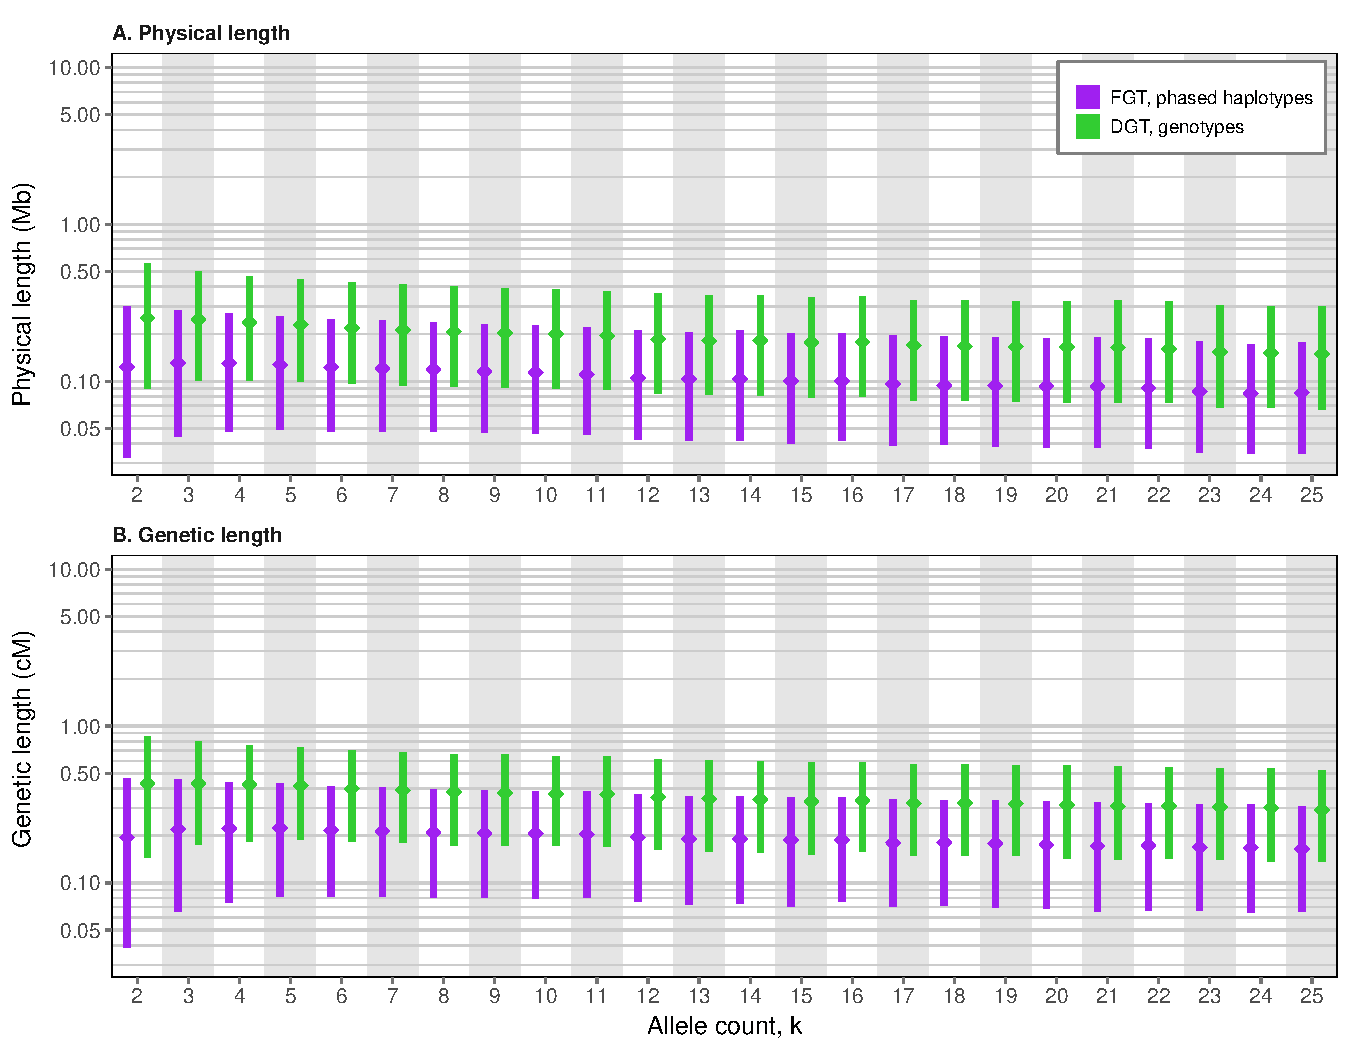
\includegraphics[width=\textwidth]{./img/ch3/length_1kg20}
\Caption{Distribution of inferred IBD lengths in 1000 Genomes data, chromosome 20}
{Results are shown for the detected physical and genetic lengths of shared haplotype segments by \fk{}, using chromosome 20 in the final release dataset of \glsentrylong{1kg} Phase~\rom{3}, including ${N = \num{2504}}$ individuals.
IBD segments were detected using the \gls{fgt} (on phased haplotypes) and the \gls{dgt} (on genotype data).
Bottom and top of each bar represent the \nth{1} and \nth{3} quartile, respectively, between which the median (\nth{2} quartile) is marked (\emph{diamonds}).}
{fig:1kg20_lengths}
\end{figure}

%

As there is no ``truth'' dataset that could serve as a reference to measure accuracy, the following analysis was limited to the quantitative description of the inferred IBD lengths.
These results are shown in \cpref{fig:1kg20_lengths}.
Median physical length (and median genetic length) over the whole set of retained IBD segments was
\SI{0.101027}{\mega\basepair} (\SI{0.1878143}{\centi\morgan}) using the \gls{fgt} and
\SI{0.179916}{\mega\basepair} (\SI{0.3393392}{\centi\morgan}) using the \gls{dgt}.
As was seen in the analysis of simulated data, the \gls{dgt} generally is more likely to overestimate breakpoint distance, leading the the discovery of longer intervals.
This discrepancy in length was more pronounced for \fk{2}~variants, for which median length was
\SI{0.1236930}{\mega\basepair} (\SI{0.1947293}{\centi\morgan}) using the \gls{fgt} and
\SI{0.2528860}{\mega\basepair} (\SI{0.4284813}{\centi\morgan}) using the \gls{dgt}.
Notably, IBD lengths were more than twice as long in half of the detected segments using the \gls{dgt}, compared to the \gls{fgt}.
The length of segments identified at lower frequencies was longer in comparison to higher frequencies; \eg for \fk{25}~variants, median length was
\SI{0.0843340}{\mega\basepair} (\SI{0.1647307}{\centi\morgan}) and
\SI{0.1492150}{\mega\basepair} (\SI{0.2918440}{\centi\morgan}) using the \gls{fgt} and \gls{dgt}, respectively.
However, the IBD lengths were highest at \fk{[3,5]} when the \gls{fgt} was used, but which was not the case for the \gls{dgt}.




\DeleteNote{Section ``Inference of the shared haplotype sequence''}
%
% %
% \subsubsection{Inference of the shared haplotype sequence}
% %
%
% The IBD-based phasing concept described in \cpref{sec:ibd_phasing} was explored in this section.
% Given the genealogical constraints that follow from the assumption that the genealogy does not change along the sequence within a given breakpoint interval, it is straightforward to derive the sequence of the shared haplotype.
% This applies to sites where exactly \n{1} genotype is heterozygous and \n{1} is homozygous in a pair of individuals.
% In the following, such heterozygous-homozygous sites are referred to as being \emph{informative}, as opposed to sites where both genotypes are heterozygous, which are referred to as being \emph{indeterminate}.
% At sites where both genotypes are homozygous, phasing is trivial.
% Hence, phasing is attempted at heterozygous sites along the sequence.
%
% The analysis was performed on the full set of IBD segments detected using the \gls{dgt} in the simulated dataset; recall that the \gls{fgt} requires (phased) haplotypes and cannot be used on genotype data.
% Also, note that breakpoint sites delimit the interval enclosing a haplotype that is shared by descent, but they themselves represent the first positions along the sequence at which haplotype sharing was broken through recombination; hence, breakpoint sites were excluded from the inference.
% The purpose of this evaluation was to determine the proportions of correctly and incorrectly phased sites, as well as the proportion of indeterminate sites.
% This was then compared to the same haplotypes inferred using the set of true IBD segments.
%
% In the following, \n{2} approaches were explored; first, haplotype inference was performed separately per IBD segment and, second, the segments identified by the same shared allele were grouped and a majority-rule was applied to determine the shared haplotype sequence (referred to as \emph{consensus} approach).
% The latter represents an attempt to increase the number of informative sites, as these may differ if more pairs of individuals are considered.
% Since they share the same focal allele, it is assumed that this allele identifies the same haplotype in all pairs.
%
% %
% %!TEX root = ../../main.tex


\begin{figure}[!htb]
\centering
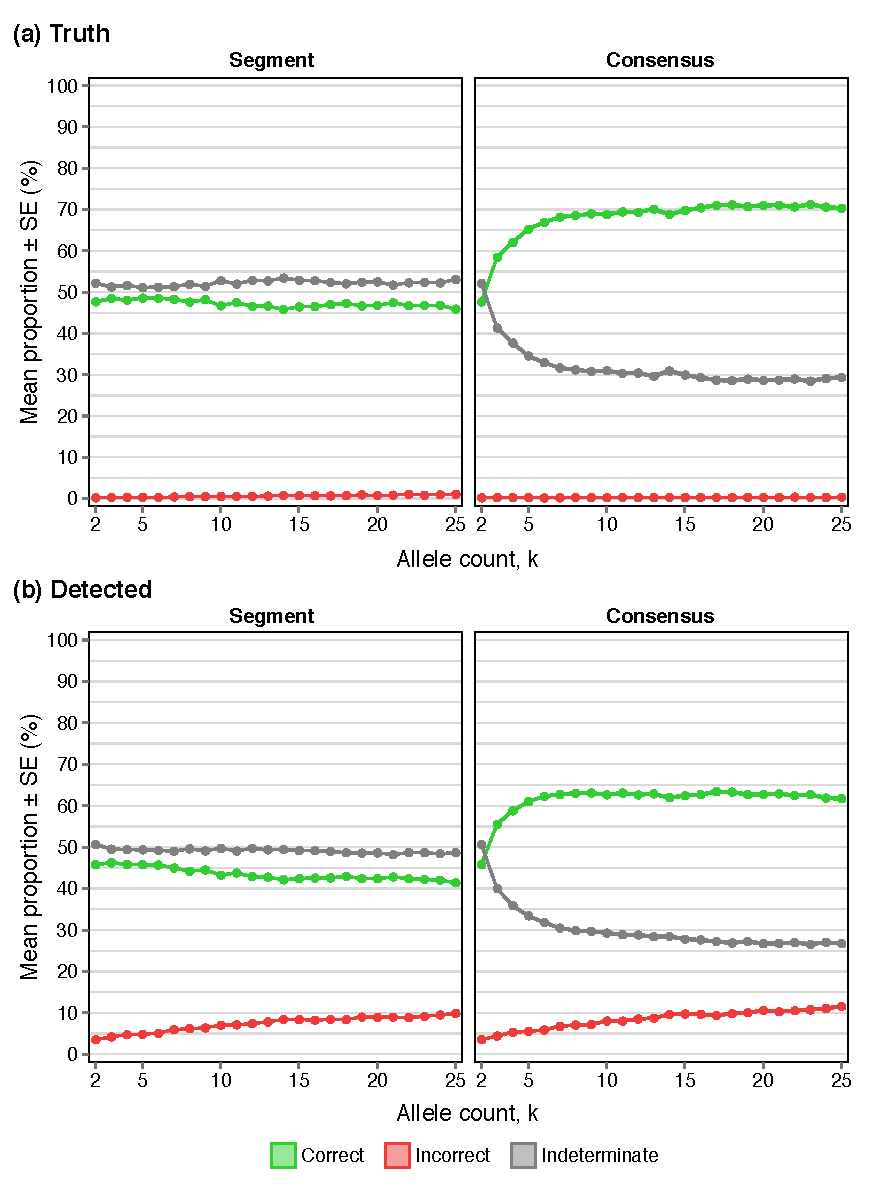
\includegraphics[width=0.75\textwidth]{./img/ch3/phase_fk_prop}
\Caption{Accuracy of alleles inferred through IBD-based phasing by focal allele frequency}
{IBD segments were randomly selected; \n{10000} per \fk{}~category.
Genotypes within each segment were phased and the relative proportions of correct, incorrect, and indeterminate alleles were recorded and averaged ($\pm\text{SE}$) per \fk{}~category.
This was done separately per segment (\emph{left}) and using the consensus approach (\emph{right}).
The results shown in Panel~\textbf{(a)} correspond to the ``truth'', where the true IBD segments were used to delimit the extent of the inferred shared haplotype sequence.
This is compared to Panel~\textbf{(b)}, where the \gls{dgt} was used to detect IBD breakpoints in genotype data.}
{fig:phase_fk_prop}
\end{figure}

% %
%
% A random subset of \n{10000} IBD segments was drawn for each \fk{}~category from the full set of detected intervals using the \gls{dgt} in which the shared haplotype was inferred.
% Similarly, for the consensus approach, target sites were randomly drawn for the set of identified targets for each \fk{}~category, such that the total number of identified segments did not exceed \n{10000} per \fk{}~category.
% Haplotypes were then inferred and combined in each focal group by applying a majority-rule to estimate the sequence of the shared haplotype.
% For each segment, the proportions of correctly inferred, incorrectly inferred, or indeterminate alleles was then determined per \fk{}~category.
% Additionally, to compare these results to the ``truth'', the same subsets of IBD segments was analysed in each approach, but where estimated haplotype length was delimited by the corresponding true IBD segments.
% The same was done for both approaches, but using the set of true IBD segments to delimit the haplotype sequence.
% The results of this analysis are shown in \cpref{fig:phase_fk_prop}.
%
% When true IBD segments were used, \cref{fig:phase_fk_prop}{a}, the proportion of incorrectly phased sites was consistently low along the allele frequency range; however, note that this proportion was not equal to zero.
% In comparison, the proportion of error increased towards higher allele frequencies when IBD was detected using the \gls{dgt}, \cref{fig:phase_fk_prop}{b}, which was seen in both the segment-based approach and the consensus approach.
% Notably, the proportion of indeterminate sites was consistently close to $50\%$ in the segment-based approach using both true and detected data.
% However, the proportion of correctly phased genotypes decreased towards higher allele frequencies; from \SI{46.173}{\percent} at \fk{2}~variants to \SI{42.330}{\percent} at \fk{25}~variants.
% In the consensus approach, the proportion of correctly phased genotypes showed a rapid increase but then reached a plateau around $70\%$ in when true IBD segments were used, and between $60\%$ and $65\%$ when detected segments were used.
%
% %
% %!TEX root = ../../main.tex


\begin{figure}[!htb]
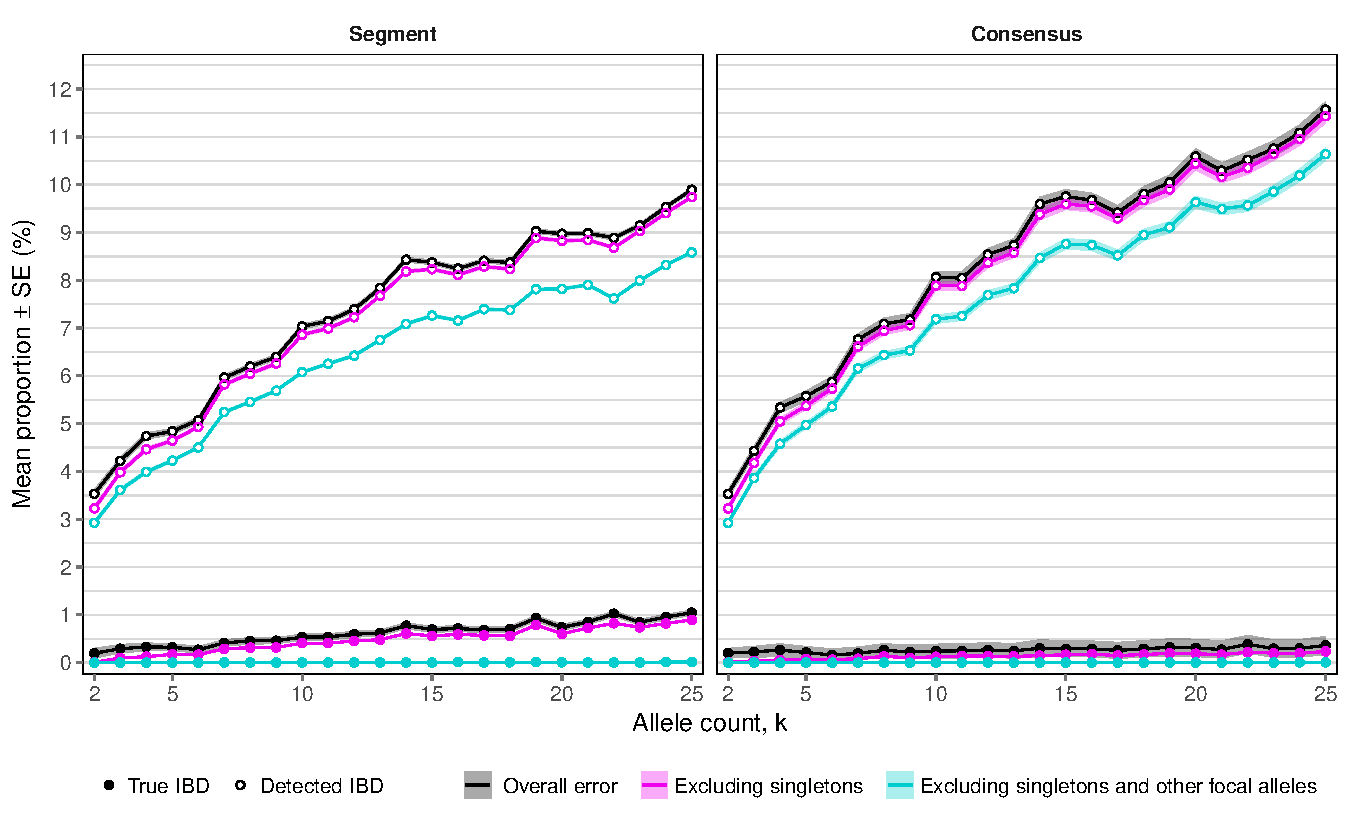
\includegraphics[width=\textwidth]{./img/ch3/phase_fk_error}
\Caption{Error distribution of alleles inferred through IBD-based phasing}
{The same results are shown as in \cref{fig:phase_fk_prop}, but with focus on incorrectly inferred alleles only; \ie the proportion of overall error corresponds to the proportion of incorrect alleles in \cref{fig:phase_fk_prop}.
The source of error was further

}
{fig:phase_fk_error}
\end{figure}

% %
%
% The distribution of incorrectly phased genotypes was further analysed to distinguish error due to singletons and other focal alleles that fell within the intervals of the segments analysed.
% These results are shown in \cpref{fig:phase_fk_error}.
% Note that in both, the exclusion of singletons did not markedly reduce the overall proportion of incorrectly phased genotypes.
% In both the segment-based approach and the consensus approach, error was noticeably reduced if genotypes at other focal variants were excluded.
% Importantly, by excluding singletons and other focal alleles that fell within the interval of the segments analysed, error was reduced to zero when true IBD segments were used.
% In fact, incorrectly phased genotypes only occurred within the overestimated regions of detected IBD segments; \ie using the \gls{dgt}.
%
% This finding is important as it suggests that haplotypes could be determined correctly if overestimation in the detection of breakpoints could be reduced or excluded.
% For example, instead of considering the full length of the segments detected, genotype phase could be determined from a narrow interval around a given target site.
%


\DeleteNote{Section ``Phasing coverage of pairwise shared haplotypes per individual''}
%
% %
% \subsubsection{Phasing coverage of pairwise shared haplotypes per individual}
% %
%
% Although the presented IBD-based phasing approach attempted to only determine genotype phase locally, it may nonetheless be of interest to explore the possibility to phase individuals ``globally''; that is, to distinguish haplotypes from genotype data along the full length of a chromosome per individual.
% To this end, it is relevant to determine the coverage of shared haplotypes along a chromosome per individual.
% Since simulated data may not be suited to derive expectations that would apply to reality, the following analysis was conducted on data from the \glsentrylong{1kg} Phase~\rom{3}, chromosome~20.
%
% I randomly selected \n{500} of the \n{2504} individuals and, for each individual, I identified all other individuals (in the whole sample of \n{2504} individuals) which shared any rare allele at \fk{[2,25]} with a given individual.
% The average number of rare alleles shared between a given individual and any other individual was \MeanValue{15234.930}{455.259586}, and the average number of unique individuals who shared any rare allele with a given individual was \MeanValue{1396.796}{9.654698}, which ranged between \n{888} and \n{1978}.
% The \gls{dgt} was used to detect segment breakpoints per pairwise shared focal allele; for comparison, the same was done using the \gls{fgt}, although only the \gls{dgt} would be applied in the context of genotype phasing.
%
% %
% %!TEX root = ../../main.tex


\begin{figure}[!htb]
%{\smaller\texthv{\textbf{A. Simulated sample}}}\\
%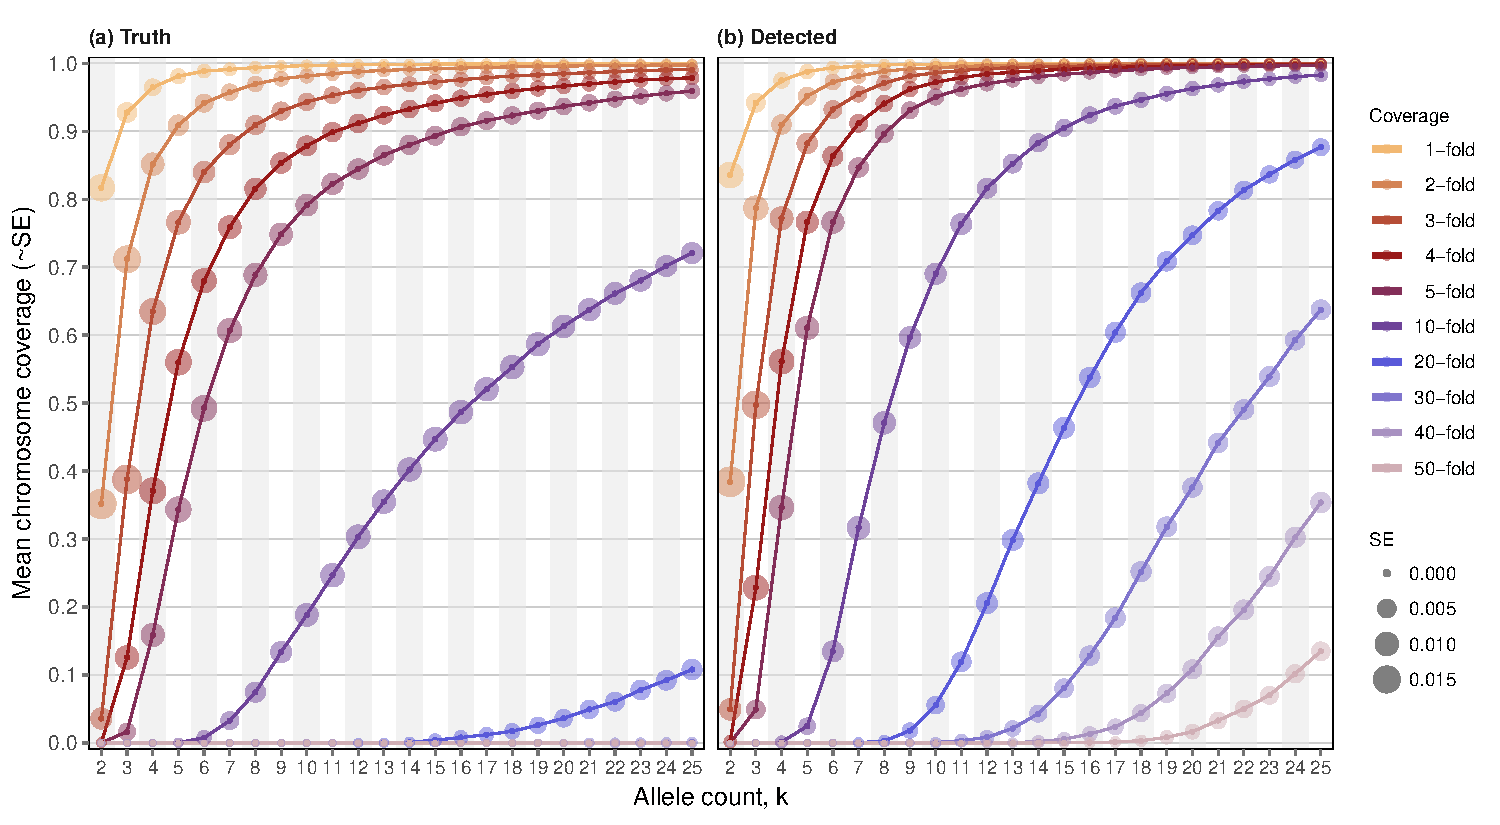
\includegraphics[width=\textwidth]{./img/ch3/phase_fk_coverage}
%{\smaller\texthv{\textbf{B. 1000 Genomes, chromosome 20}}}\\
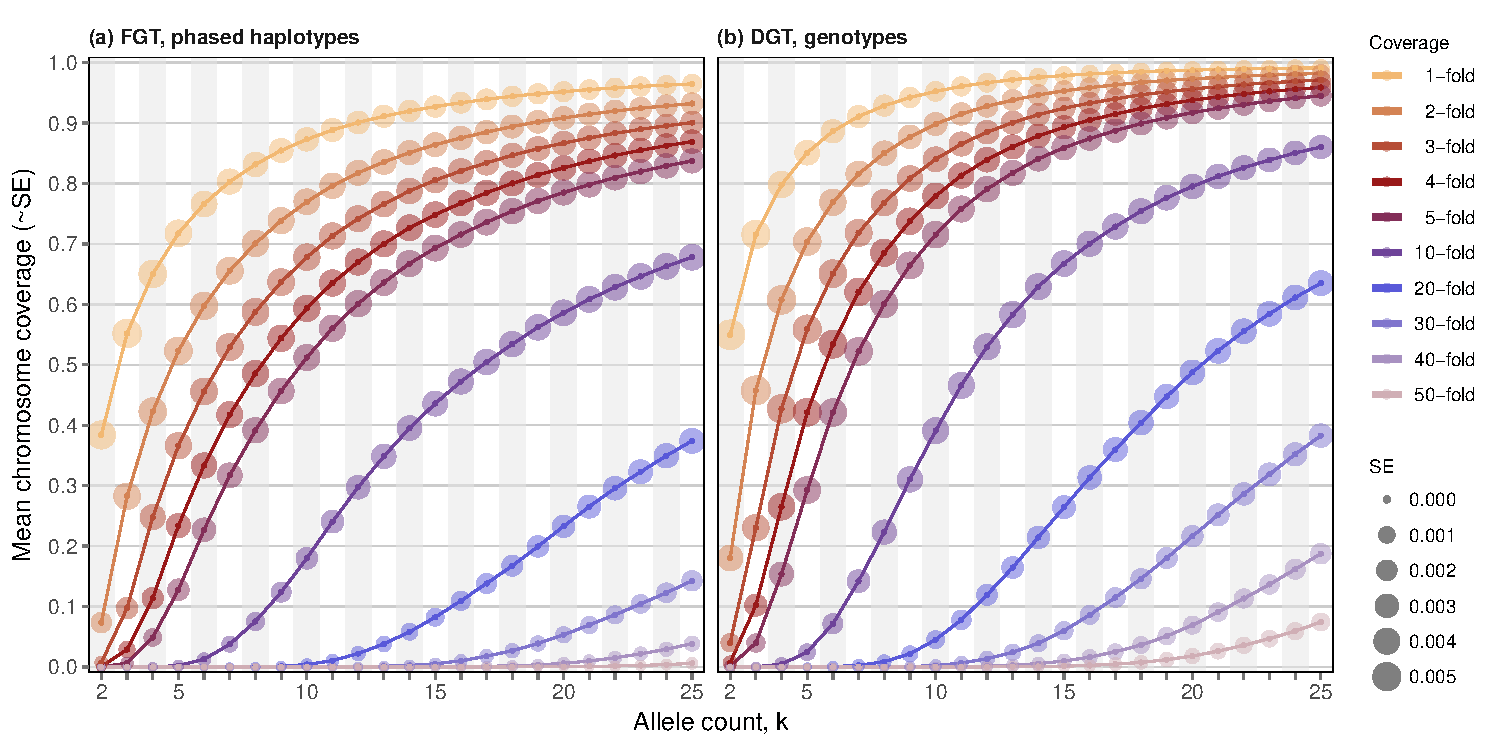
\includegraphics[width=\textwidth]{./img/ch3/phase_coverage_1kg}
\Caption{Cumulative shared haplotype coverage by focal allele count in 1000 Genomes data}
{Results are shown for \n{500} randomly selected individuals, among ${N=\num{2504}}$ in the \gls{1kg} dataset.
% (\textbf{A}), and among the ${N=\num{2504}}$ individuals in 1000 Genomes data, chromosome~20 (\textbf{B}).
Segments detected using the \gls{fgt} (\text{a}, \emph{left}) are compared to the segments detected using the \gls{dgt} (\text{b}, \emph{right}).
%In~B, for comparison, the \gls{fgt} is compared to the \gls{dgt} in the 1000 Genomes dataset.
Coverage was defined as the proportion of chromosome length covered by inferred and aligned shared haplotypes, where $n$-fold indicates that the chromosome was covered $n$-times by all segments up to a given \fk{}~category (hence, cumulative).
\Gls{se} is indicated by the size of dots (see figure legend).}
{fig:phase_fk_coverage}
\end{figure}

% %
%
% Each set of detected segments was then reduced to include only unique IBD intervals; again after sorting by focal allele frequency such that the focal allele is the one with lowest frequency within a given segment.
% Recall that duplicate segments refer to IBD intervals that are tagged by multiple \fk{}~variants, which are assumed to sit on the same underlying shared haplotype.
% The average number of unique segments retained per individual was \MeanValue{5071.224}{79.976994} for the \gls{dgt} and \MeanValue{5460.694}{85.317616} for the \gls{fgt}; note that haplotype data were phased.
% Retained haplotype segments were aligned by position along the chromosome to measure coverage, \ie the proportion of the chromosome covered.
% Mean coverage across all \n{500} randomly selected individuals is given in \cpref{fig:phase_fk_coverage}, which indicates the $n$-fold cumulative coverage by \fk{}~category; shown for true IBD segments (\cref{fig:phase_fk_coverage}{a}) and segments detected using the \gls{dgt} (\cref{fig:phase_fk_coverage}{b}).
%
% Coverage was overall higher for the \gls{dgt} compared to the \gls{fgt}, due to overestimating IBD lengths.
% Notably, neither the \gls{dgt} nor the \gls{fgt} reached full coverage on average.
% However, a steady increase was seen when \fk{}~variants at higher frequency were included.
% Considering \fk{2}~variants alone, the \gls{dgt} reached ${>50\%}$ 1-fold coverage, which was higher compared to the \gls{fgt} with ${< 40\%}$ 1-fold coverage.
% Considering focal alleles occurring at higher frequencies, the \gls{dgt} was at ${\approx 99\%}$ 1-fold cummulative coverage at \fk{\leq 20}, whereas the \gls{fgt} slowly approached ${\approx 95\%}$ 1-fold cummulative coverage at \fk{\leq 25}.
%
% These results indicate that a ``global'' phasing approach using inferred IBD information alone would not be able to fully determine haplotypes in sample data of unrelated individuals.
% However, note that similar approaches have been applied to sets of related individuals, for which it can be expected that there are more and longer pairwise shared haplotypes; \ie \glsentryfull{lrp} methods \citep{Kong:2008gh,Palin:2011cl,loh2016fast}.
%



%
\section{Discussion}
%


In this chapter, I presented a novel IBD detection method which is able to infer recombination events in both haplotype and genotype data.
To be able to apply this method on a larger scale, I implemented the IBD detection algorithm described in this chapter as a computational tool written in \cpp; called \textbf{\texttt{tidy}} (\underline{t}argeted \underline{I}BD \underline{d}etection done thoroughl\underline{y}).\footnote{Targeted IBD detection done thoroughly, \texttt{tidy}: \url{https://github.com/pkalbers/tidy}}
% I applied the \texttt{tidy} algorithm to all autosomes in the \gls{1kg} dataset, in which I included all rare allele \glspl{snp} observed below a $0.5$\% allele frequency threshold (\ie \fk{}~variants with ${k \in [2, 25]}$).
% This was done using both the \gls{fgt} and the \gls{dgt}; the results are available online.\footnote{Download ???}

Although the \gls{fgt} showed overall high levels of accuracy, phasing error was identified as a problem.
Current phasing methods such as \texttt{SHAPEIT\,2} typically show very low error rates \citep{OConnell:2014fl}.
However, occasionally, alleles are placed on the wrong haplotype.
This may happen at single loci (\emph{flip~errors}) or such that longer haplotype stretches are exchanged (\emph{switch~errors}).
Both types of error can affect breakpoint detection under the \gls{fgt} as both flip and switch errors may change the configuration of alleles observed in relation to a given focal variant.
As an alternate solution to using phased haplotypes, the \gls{dgt} can be used on genotype data, which is therefore not affected by phasing error.
However, the lengths of detected IBD segments tend to be overestimated.

Notably, the IBD results obtained from analysis of the \gls{1kg} dataset suggests that the \gls{fgt} was similarly affected by phasing error as seen in the simulation analysis.
However, the \gls{dgt} was also affected by other sources of error.
One consideration is that both the \gls{fgt} and \gls{dgt} assume the infinite sites model, but this is only an approximation of conditions observable in nature.
In particular, back mutations and recurrent mutations are excluded in the model, but these are prevalent in the (human) genome.
For instance, recurrent mutations can produce patterns of variation that would otherwise only be observable if recombination had occurred \citep{McVean:2002ws}.
Thus, false positive breakpoints may be inferred, such that IBD length is underestimated.
Nonetheless, the infinite sites model is usually seen as a reasonable approximation to reality, as the number of variant sites in a sample is typically much smaller than the number of nucleotides in the chromosomal sequence \citep{hein2004gene}.
However, the presence of genotype error cannot be ruled out and therefore requires further consideration.


\Delete{
Lastly, the IBD-based phasing concept showed that that it is possible to derive the shared allelic state sequence in pairs of individuals that share a haplotype by descent.
This approach, in its current implementation, is only able to phase genotype data over locally shared segments.
However, a potential utility of such a local phasing approach may arise considering that rare variants can be used to identify recent relatedness patterns in large datasets.
Because a given rare allele identifies the underlying shared haplotype, the inferred sequence is likely to correctly distinguish the haplotypes of an individual within a shorter region around the target position.
For example, this information may serve as a \emph{post-hoc} correction to haplotype data produced using existing phasing methods.
}
